% !TEX program = xelatex
% Компилира се с XeLaTeX:  xelatex lekciya.tex  (два пъти, заради съдържанието)
\documentclass[11pt,a4paper]{article}
\usepackage[a4paper,left=2.1cm,right=2.1cm,top=2.2cm,bottom=2.3cm]{geometry}
\usepackage{amsmath}
\usepackage{unicode-math}
\setmainfont{Fira Sans}[BoldFont={Fira Sans SemiBold}]
\setsansfont{Fira Sans}[BoldFont={Fira Sans SemiBold}]
\setmonofont{DejaVu Sans Mono}[Scale=0.84]
\setmathfont{Latin Modern Math}[Scale=MatchLowercase]
\setmathfont{Fira Sans}[range={up/num}]

\usepackage{xcolor}
\definecolor{ink}{HTML}{17191C}
\definecolor{cblue}{HTML}{0866F5}
\definecolor{corange}{HTML}{B85B24}
\definecolor{cgreen}{HTML}{297D55}
\definecolor{cpurple}{HTML}{7256AC}
\definecolor{cred}{HTML}{C2332B}
\definecolor{soft}{HTML}{F4F5F2}
\definecolor{muted}{HTML}{6B6E69}
\color{ink}

\usepackage{tikz}
\usetikzlibrary{arrows.meta,positioning,calc,shapes.geometric,decorations.pathreplacing}
\usepackage{pgfplots}
\pgfplotsset{compat=1.18}
\usepackage[most]{tcolorbox}
\usepackage{fancyvrb}
\usepackage{enumitem}
\usepackage{array,booktabs}
\usepackage{multicol}
\usepackage{fancyhdr}
\usepackage{titlesec}
\usepackage{etoolbox}
\usepackage{needspace}
\usepackage[colorlinks=true,linkcolor=cblue,urlcolor=cblue]{hyperref}
\makeatletter\def\@minipagerestore{\raggedright\setlength{\parskip}{5pt}}\makeatother
\tcbset{halign=flush left,before upper={\setlength{\parskip}{4pt}}}
\fvset{listparameters={\setlength{\topsep}{1pt}\setlength{\partopsep}{0pt}}}

\raggedright
\setlength{\parindent}{0pt}
\setlength{\parskip}{6pt plus 2pt}
\linespread{1.08}
\setlist{itemsep=2pt,topsep=3pt,leftmargin=1.5em}
\renewcommand{\contentsname}{Съдържание}
\renewcommand{\figurename}{Фигура}

% ---------- заглавия ----------
\titleformat{\section}{\Large\bfseries\color{ink}}{\textcolor{cblue}{\thesection}}{0.6em}{}
\titleformat{\subsection}{\large\bfseries\color{ink}}{}{0pt}{}
\titlespacing*{\section}{0pt}{16pt}{6pt}
\titlespacing*{\subsection}{0pt}{12pt}{3pt}

\pagestyle{fancy}\fancyhf{}
\renewcommand{\headrulewidth}{0pt}
\fancyfoot[L]{\footnotesize\color{muted}AI клуб · ТУЕС · Начинаещи · Урок 4: Функции}
\fancyfoot[R]{\footnotesize\color{muted}\thepage}

% ---------- карета ----------
\newtcolorbox{defbox}[1][Определение]{enhanced,breakable,colback=cblue!5,colframe=cblue,boxrule=0pt,leftrule=3.5pt,
  arc=2pt,left=9pt,right=9pt,top=6pt,bottom=6pt,fonttitle=\bfseries\small,coltitle=cblue,
  attach title to upper={\par\vspace{1pt}},title={#1}}
\newtcolorbox{board}{enhanced,breakable,colback=white,colframe=ink,boxrule=1.1pt,arc=3pt,
  left=10pt,right=10pt,top=7pt,bottom=7pt,fonttitle=\bfseries\small,coltitle=white,colbacktitle=ink,
  title={На дъската},attach boxed title to top left={xshift=8pt,yshift=-9pt},
  boxed title style={arc=2pt,boxrule=0pt,left=5pt,right=5pt,top=2pt,bottom=2pt},top=13pt}
\newtcolorbox{trybox}{enhanced,breakable,colback=corange!7,colframe=corange,boxrule=0pt,leftrule=3.5pt,
  arc=2pt,left=9pt,right=9pt,top=6pt,bottom=6pt,fonttitle=\bfseries\small,coltitle=corange,
  attach title to upper={\par\vspace{1pt}},title={Провери се}}
\newtcolorbox{pybox}{enhanced,colback=cgreen!6,colframe=cgreen,boxrule=0pt,leftrule=3.5pt,
  arc=2pt,left=9pt,right=9pt,top=6pt,bottom=4pt,fonttitle=\bfseries\small,coltitle=cgreen,
  attach title to upper={\par\vspace{1pt}},title={Същото на Python}}
\newtcolorbox{funbox}[1][За любопитните]{enhanced,breakable,colback=cpurple!6,colframe=cpurple,boxrule=0pt,leftrule=3.5pt,
  arc=2pt,left=9pt,right=9pt,top=6pt,bottom=6pt,fonttitle=\bfseries\small,coltitle=cpurple,
  attach title to upper={\par\vspace{1pt}},title={#1}}
\newcommand{\level}[1]{\textcolor{corange}{#1}}
\newcommand{\grp}[2]{\par\vspace{8pt}{\large\bfseries\textcolor{cblue}{#1}\hspace{0.5em}#2}\par\vspace{2pt}}
\newcommand{\st}{\textcolor{corange}{$\star$}}
\newlist{tasks}{enumerate}{1}
\setlist[tasks]{label=\textbf{\arabic*.},leftmargin=2.2em,itemsep=7pt,topsep=4pt,resume}
\makeatletter
\newcommand{\bgalph}[1]{\expandafter\@bgalph\csname c@#1\endcsname}
\newcommand{\@bgalph}[1]{\ifcase#1\or а\or б\or в\or г\or д\or е\or ж\or з\or и\or к\fi}
\AddEnumerateCounter{\bgalph}{\@bgalph}{м}
\makeatother
\newcommand{\blank}{\rule{0.9cm}{0.4pt}}
\newcommand{\figcap}[1]{\par\vspace{2pt}{\small\color{muted}#1}\par}

% ---------- графики ----------
\pgfplotsset{
  fgraph/.style={
    axis lines=middle,
    axis line style={-{Stealth[length=5pt]},line width=.7pt,draw=ink},
    grid=both, grid style={line width=.3pt,draw=black!13},
    xtick distance=1, ytick distance=1,
    tick style={draw=none},
    tick label style={font=\scriptsize,text=muted},
    xlabel={$x$}, ylabel={$y$},
    xlabel style={at={(ticklabel* cs:1)},anchor=north west,font=\small},
    ylabel style={at={(ticklabel* cs:1)},anchor=south west,font=\small},
    every axis plot/.append style={line width=1.3pt,samples=121,smooth},
    x=0.62cm, y=0.62cm, clip=true, clip mode=individual,
    legend style={draw=none,fill=white,fill opacity=.9,text opacity=1,font=\small,cells={anchor=west}},
  },
  pt/.style={only marks,mark=*,mark size=2.1pt},
  mini/.style={x=0.44cm,y=0.44cm,tick label style={font=\tiny,text=muted}},
}
\tikzset{
  mach/.style={draw=cblue,line width=1.1pt,fill=cblue!7,rounded corners=4pt,minimum width=3.4cm,minimum height=1.5cm,align=center},
  io/.style={font=\large},
  arr/.style={-{Stealth[length=6pt]},line width=1pt,draw=ink},
  lab/.style={font=\scriptsize,fill=white,fill opacity=.88,text opacity=1,inner sep=1.5pt},
}
\begin{document}

% ================= заглавна част =================
{\small\bfseries\color{cblue} AI КЛУБ · ТУЕС · НАЧИНАЕЩИ · УРОК 4}\par\vspace{2pt}
{\fontsize{30}{34}\selectfont\bfseries Функции}\par\vspace{4pt}
{\large Какво е функция, как се чете графика и кои функции ще срещаме най-често}\par
\vspace{8pt}

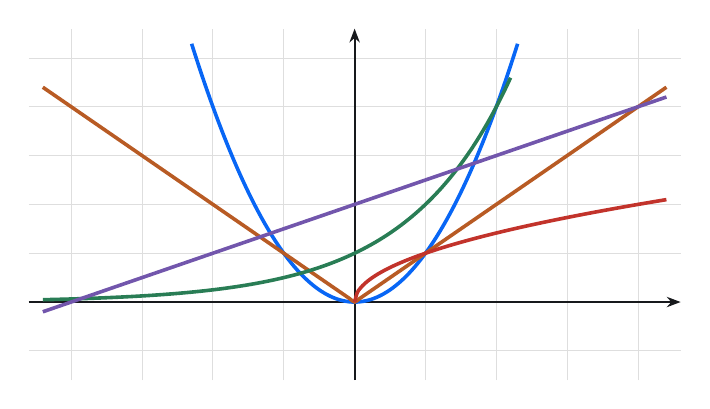
\begin{tikzpicture}
\begin{axis}[fgraph,xmin=-4.6,xmax=4.6,ymin=-1.6,ymax=5.6,x=0.9cm,y=0.62cm,xlabel={},ylabel={},
  xticklabels={},yticklabels={}]
\addplot[cblue,domain=-2.3:2.3]{x^2};
\addplot[corange,domain=-4.4:4.4]{abs(x)};
\addplot[cgreen,domain=-4.4:2.2]{2^x};
\addplot[cpurple,domain=-4.4:4.4]{0.5*x+2};
\addplot[cred,domain=0:4.4]{sqrt(x)};
\end{axis}
\end{tikzpicture}

\vspace{4pt}
\textbf{Защо учим това в клуб по изкуствен интелект?} Защото всеки модел е функция: получава числа и връща числа.
Ако разбираме функциите, разбираме какво прави моделът. А и функциите в Python са същата идея, записана с код.

\textbf{Как да четеш този материал.} В черните карета \textbf{„На дъската“} е най-важното от всяка част.
В оранжевите карета \textbf{„Провери се“} има кратки въпроси, а отговорите им са на стр.~\pageref{sec:answers}.
Зелените карета показват същото на Python. Накрая има задачи за час и за домашно.

\setcounter{tocdepth}{1}
{\small\setlength{\parskip}{0pt}
\raggedcolumns\begin{multicols}{2}[\subsection*{Съдържание}]
\makeatletter\@starttoc{toc}\makeatother
\end{multicols}}

\newpage
% =====================================================================
\section{Какво е функция}

Представи си машинка. Пускаш в нея число, тя прави с него винаги едно и също и ти връща друго число.

\begin{center}
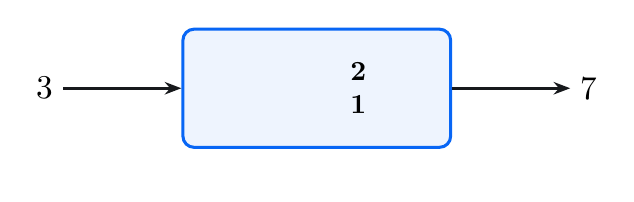
\begin{tikzpicture}
\node[io] (in) at (0,0) {$3$};
\node[mach,right=1.5cm of in] (m) {\textbf{умножи по 2}\\\textbf{и прибави 1}};
\node[io,right=1.5cm of m] (out) {$7$};
\draw[arr] (in) -- node[above,font=\small,text=muted]{вход} (m);
\draw[arr] (m) -- node[above,font=\small,text=muted]{изход} (out);
\node[below=2pt of m,font=\small,text=cblue] {правило};
\end{tikzpicture}
\end{center}

Ако пуснем $0$, излиза $1$. Ако пуснем $-2$, излиза $-3$. Ако пуснем пак $3$, пак излиза $7$. Машинката никога не си променя решението.

\begin{defbox}
\textbf{Функция} е правило, което на всеки позволен вход съпоставя \textbf{точно един} изход.
\end{defbox}

\subsection{Как записваме функция}

Вместо да рисуваме машинка, пишем кратко:
\[ f(x) = 2x + 1 \]
Чете се „еф от хикс е равно на две хикс плюс едно“. Всяка част от записа значи нещо:

\begin{center}
\begin{tikzpicture}[every node/.style={font=\Large}]
\node (f) at (0,0) {$f$};
\node[right=-1pt of f] (p1) {$($};
\node[right=-3pt of p1] (x) {$x$};
\node[right=-3pt of x] (p2) {$)$};
\node[right=2pt of p2] (eq) {$=$};
\node[right=2pt of eq] (r) {$2x+1$};
\node[below left=0.9cm and 0.5cm of f,font=\small,text=cblue,align=center] (nf) {име на\\функцията};
\node[below=0.9cm of x,font=\small,text=corange,align=center] (nx) {вход};
\node[below right=0.9cm and 0.1cm of r,font=\small,text=cgreen,align=center] (nr) {правило:\\какво правим с входа};
\draw[cblue,-{Stealth[length=4pt]}] (nf) -- (f);
\draw[corange,-{Stealth[length=4pt]}] (nx) -- (x);
\draw[cgreen,-{Stealth[length=4pt]}] (nr) -- (r);
\end{tikzpicture}
\end{center}

За да намерим изхода, слагаме числото на мястото на $x$:
\[ f(3) = 2\cdot 3 + 1 = 7 \qquad f(0) = 2\cdot 0 + 1 = 1 \qquad f(-2) = 2\cdot(-2) + 1 = -3 \]

Записът $f(3)$ се чете „еф от три“ и означава \textbf{изхода}, който функцията дава при вход $3$.
Името не е задължително да е $f$. Често ползваме и $g$, $h$ или цели думи.

\begin{pybox}
\begin{Verbatim}
def f(x):
    return 2 * x + 1

print(f(3))     # 7
print(f(-2))    # -3
\end{Verbatim}
Името е \texttt{f}, входът е параметърът \texttt{x}, а \texttt{return} връща изхода. Нищо ново, само друг запис.
\end{pybox}

\subsection{Таблица със стойности}

Удобно е да подредим няколко входа и техните изходи в таблица. За $f(x)=2x+1$:

\begin{center}
\renewcommand{\arraystretch}{1.25}
\begin{tabular}{>{\bfseries}c|*{6}{>{\centering\arraybackslash}p{0.9cm}}}
вход $x$ & $-2$ & $-1$ & $0$ & $1$ & $2$ & $3$\\\hline
изход $f(x)$ & $-3$ & $-1$ & $1$ & $3$ & $5$ & $7$
\end{tabular}
\end{center}

\subsection{Кога едно правило не е функция}

Думите „точно един изход“ са важни. Нека сравним две правила.

\begin{center}
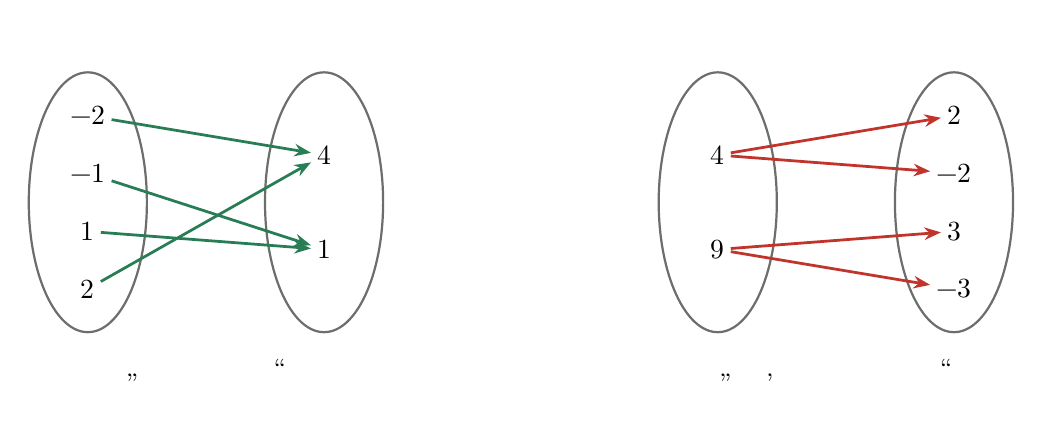
\begin{tikzpicture}[
  el/.style={font=\normalsize,inner sep=2pt},
  set/.style={draw=muted,line width=.8pt,ellipse,minimum width=1.5cm,minimum height=3.3cm}]
% --- функция ---
\node[set] at (0,0) {}; \node[set] at (3,0) {};
\foreach \y/\v in {1.1/-2,0.37/-1,-0.37/1,-1.1/2} \node[el] (a\v) at (0,\y) {$\v$};
\node[el] (b4) at (3,0.6) {$4$}; \node[el] (b1) at (3,-0.6) {$1$};
\draw[arr,cgreen] (a-2) -- (b4); \draw[arr,cgreen] (a2) -- (b4);
\draw[arr,cgreen] (a-1) -- (b1); \draw[arr,cgreen] (a1) -- (b1);
\node[font=\small\bfseries,text=cgreen] at (1.5,2.1) {функция};
\node[font=\small,align=center] at (1.5,-2.3) {„повдигни на квадрат“\\от всеки вход излиза една стрелка};
% --- не е функция ---
\begin{scope}[xshift=8cm]
\node[set] at (0,0) {}; \node[set] at (3,0) {};
\node[el] (c4) at (0,0.6) {$4$}; \node[el] (c9) at (0,-0.6) {$9$};
\foreach \y/\v in {1.1/2,0.37/-2,-0.37/3,-1.1/-3} \node[el] (d\v) at (3,\y) {$\v$};
\draw[arr,cred] (c4) -- (d2); \draw[arr,cred] (c4) -- (d-2);
\draw[arr,cred] (c9) -- (d3); \draw[arr,cred] (c9) -- (d-3);
\node[font=\small\bfseries,text=cred] at (1.5,2.1) {не е функция};
\node[font=\small,align=center] at (1.5,-2.3) {„число, чийто квадрат е входът“\\от един вход излизат две стрелки};
\end{scope}
\end{tikzpicture}
\end{center}

Вляво два различни входа ($-2$ и $2$) дават един и същ изход. Това е позволено.
Вдясно един вход дава два различни изхода. Това не е позволено, защото машинката трябва винаги да знае какво да върне.

Същото важи и извън математиката. „На всеки ученик съпоставяме рождената му дата“ е функция.
„На всеки ученик съпоставяме негов приятел“ не е, защото приятелите може да са няколко.

\begin{board}
\textbf{Функция:} правило, което на всеки вход дава точно един изход.\\[2pt]
$f(x)=2x+1$ \quad $f(3)=2\cdot 3+1=7$ \quad $f(0)=1$ \quad $f(-2)=-3$\\[2pt]
Два входа може да имат един изход. Един вход не може да има два изхода.
\end{board}

\begin{trybox}
\begin{enumerate}[label=\textbf{\arabic*.}]
  \item Нека $g(x)=x^2-1$. Намери $g(3)$, $g(0)$ и $g(-3)$.
  \item Нека $h(x)=10-x$. За кое $x$ е вярно $h(x)=6$?
  \item Функция ли е правилото „на всяко цяло число съпоставяме следващото цяло число“?
\end{enumerate}
\end{trybox}

% =====================================================================
\section{От таблица към графика}

Таблицата показва само няколко входа. Графиката показва всички наведнъж.

Всяка колона от таблицата е една точка: входът $x$ е първата координата, а изходът $f(x)$ е втората.
За $f(x)=2x+1$ колоната „вход $1$, изход $3$“ е точката $(1,3)$.

\begin{center}
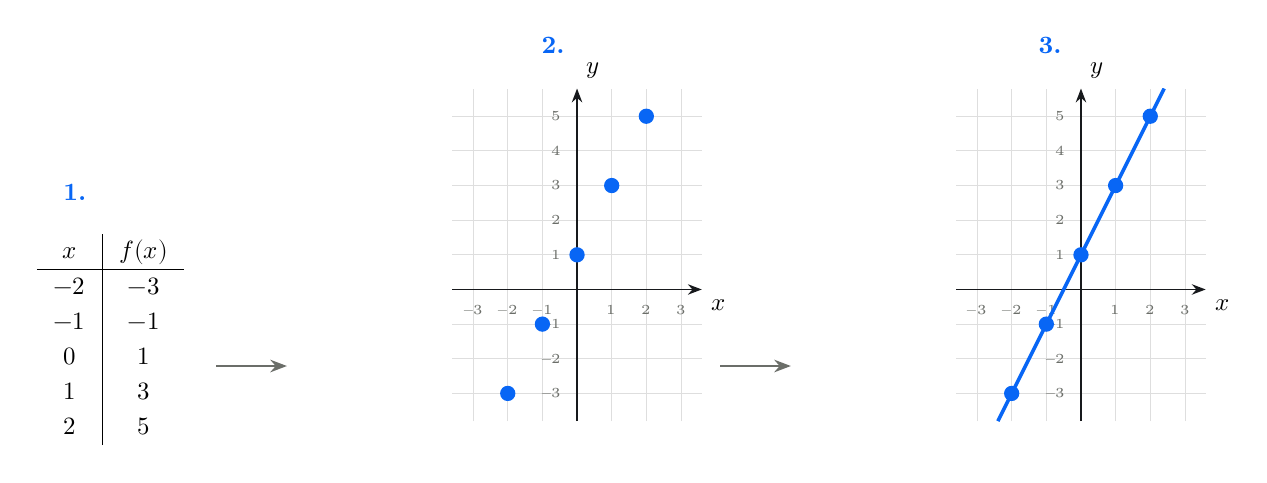
\begin{tikzpicture}
% таблица
\node[anchor=north west] at (-0.3,3.9) {\small\renewcommand{\arraystretch}{1.15}%
\begin{tabular}{c|c}
$x$ & $f(x)$\\\hline $-2$ & $-3$\\ $-1$ & $-1$\\ $0$ & $1$\\ $1$ & $3$\\ $2$ & $5$
\end{tabular}};
\node[font=\small\bfseries,text=cblue] at (0.7,4.3) {1. Таблица};
\draw[arr,muted] (2.1,2.1) -- (3.0,2.1);
\begin{scope}[xshift=5.1cm,yshift=1.4cm]
\begin{axis}[fgraph,mini,xmin=-3.6,xmax=3.6,ymin=-3.8,ymax=5.8,name=A]
\addplot[pt,cblue] coordinates {(-2,-3)(-1,-1)(0,1)(1,3)(2,5)};
\end{axis}
\node[font=\small\bfseries,text=cblue] at ($(A.north)+(0,0.55)$) {2. Точки};
\end{scope}
\draw[arr,muted] (8.5,2.1) -- (9.4,2.1);
\begin{scope}[xshift=11.5cm,yshift=1.4cm]
\begin{axis}[fgraph,mini,xmin=-3.6,xmax=3.6,ymin=-3.8,ymax=5.8,name=B]
\addplot[cblue,domain=-2.4:2.4]{2*x+1};
\addplot[pt,cblue] coordinates {(-2,-3)(-1,-1)(0,1)(1,3)(2,5)};
\end{axis}
\node[font=\small\bfseries,text=cblue] at ($(B.north)+(0,0.55)$) {3. Графика};
\end{scope}
\end{tikzpicture}
\end{center}

Между целите числа има и други входове, например $0{,}5$ или $1{,}5$. Те също дават точки и всички заедно запълват линията.

\begin{defbox}
\textbf{Графиката} на функцията $f$ са всички точки $(x, f(x))$.
Хоризонталната ос показва входа, вертикалната показва изхода.
\end{defbox}

\subsection{Как се чете графика}

\begin{minipage}[c]{0.47\textwidth}
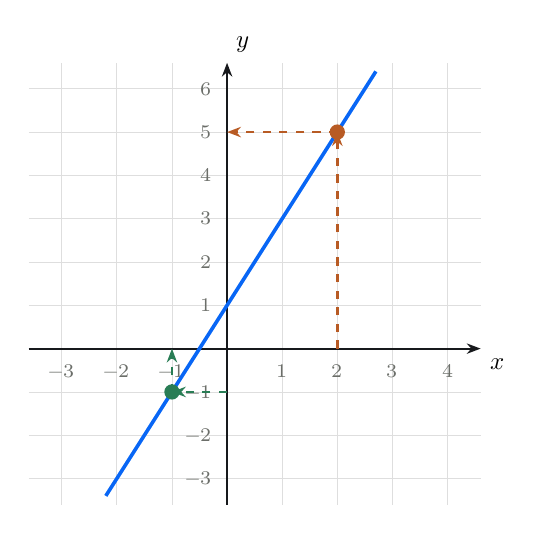
\begin{tikzpicture}
\begin{axis}[fgraph,xmin=-3.6,xmax=4.6,ymin=-3.6,ymax=6.6,x=0.7cm,y=0.55cm]
\addplot[cblue,domain=-2.2:2.7]{2*x+1};
\draw[corange,line width=1pt,dashed,-{Stealth[length=5pt]}] (axis cs:2,0) -- (axis cs:2,5);
\draw[corange,line width=1pt,dashed,-{Stealth[length=5pt]}] (axis cs:2,5) -- (axis cs:0,5);
\addplot[pt,corange] coordinates {(2,5)};
\draw[cgreen,line width=1pt,dashed,-{Stealth[length=5pt]}] (axis cs:0,-1) -- (axis cs:-1,-1);
\draw[cgreen,line width=1pt,dashed,-{Stealth[length=5pt]}] (axis cs:-1,-1) -- (axis cs:-1,0);
\addplot[pt,cgreen] coordinates {(-1,-1)};
\end{axis}
\end{tikzpicture}
\end{minipage}\hfill
\begin{minipage}[c]{0.5\textwidth}
\textbf{\textcolor{corange}{От вход към изход.}} Колко е $f(2)$?
Тръгваме от $2$ на оста $x$, качваме се до графиката и поглеждаме наляво към оста $y$. Получаваме $5$.

\vspace{6pt}
\textbf{\textcolor{cgreen}{От изход към вход.}} За кое $x$ е вярно $f(x)=-1$?
Тръгваме от $-1$ на оста $y$, отиваме до графиката и поглеждаме към оста $x$. Получаваме $x=-1$.
\end{minipage}

\subsection{Всяка линия ли е графика на функция}

Не. Ако някоя вертикална права пресича линията на две места, значи един вход има два изхода. Тогава линията не е графика на функция.

\begin{center}
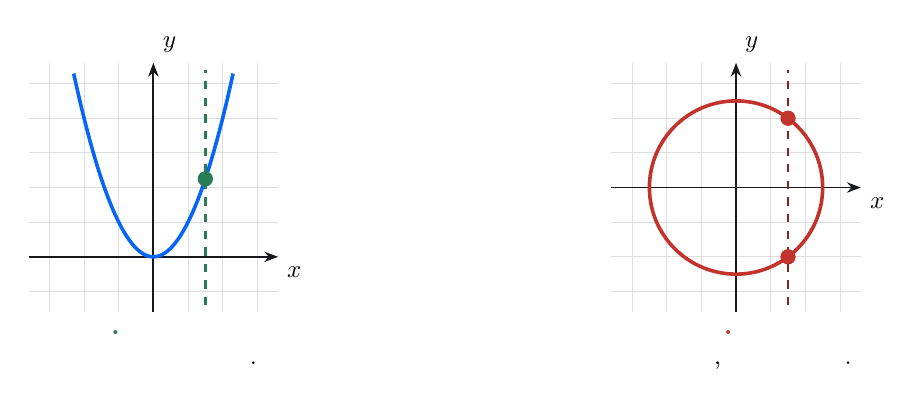
\begin{tikzpicture}
\begin{axis}[fgraph,mini,xmin=-3.6,xmax=3.6,ymin=-1.6,ymax=5.6,name=A,xticklabels={},yticklabels={}]
\addplot[cblue,domain=-2.3:2.3]{x^2};
\draw[cgreen,line width=1pt,dashed] (axis cs:1.5,-1.4) -- (axis cs:1.5,5.4);
\addplot[pt,cgreen] coordinates {(1.5,2.25)};
\end{axis}
\node[font=\small,align=center,below=3pt of A] {\textbf{\textcolor{cgreen}{Функция.}} Всяка вертикална\\права пресича линията веднъж.};
\begin{scope}[xshift=7.4cm]
\begin{axis}[fgraph,mini,xmin=-3.6,xmax=3.6,ymin=-3.6,ymax=3.6,name=B,xticklabels={},yticklabels={}]
\draw[cred,line width=1.3pt] (axis cs:0,0) circle [radius=2.5];
\draw[cred!70!black,line width=1pt,dashed] (axis cs:1.5,-3.4) -- (axis cs:1.5,3.4);
\addplot[pt,cred] coordinates {(1.5,2)(1.5,-2)};
\end{axis}
\node[font=\small,align=center,below=3pt of B] {\textbf{\textcolor{cred}{Не е функция.}} При един вход\\има две точки, тоест два изхода.};
\end{scope}
\end{tikzpicture}
\end{center}

\begin{board}
Графика: всички точки $(x, f(x))$. Ос $x$ е входът, ос $y$ е изходът.\\[2pt]
Таблица $\rightarrow$ точки $\rightarrow$ линия.\\[2pt]
Вертикална права пресича графиката на функция най-много веднъж.
\end{board}

\begin{trybox}
\begin{minipage}[c]{0.4\textwidth}
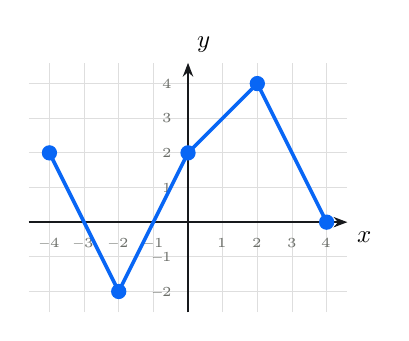
\begin{tikzpicture}
\begin{axis}[fgraph,mini,xmin=-4.6,xmax=4.6,ymin=-2.6,ymax=4.6]
\addplot[cblue,sharp plot] coordinates {(-4,2)(-2,-2)(0,2)(2,4)(4,0)};
\addplot[pt,cblue] coordinates {(-4,2)(-2,-2)(0,2)(2,4)(4,0)};
\end{axis}
\end{tikzpicture}
\end{minipage}\hfill
\begin{minipage}[c]{0.56\textwidth}
Това е графиката на функция $f$.
\begin{enumerate}[label=\textbf{\arabic*.},start=4]
  \item Колко е $f(-2)$? А $f(0)$? А $f(3)$?
  \item За кои $x$ е вярно $f(x)=0$?
  \item Коя е най-голямата стойност на функцията и при кое $x$ се получава?
\end{enumerate}
\end{minipage}
\end{trybox}

% =====================================================================
\section{Позволени входове}

Някои функции не могат да работят с всяко число.

\begin{itemize}
  \item $f(x)=\sqrt{x}$ работи само за $x\ge 0$. Корен от $-4$ няма, защото никое число на квадрат не дава $-4$.
  \item $f(x)=\dfrac{12}{x}$ не работи за $x=0$, защото на нула не се дели.
  \item Ако $x$ е брой билети, позволени са само целите числа $0, 1, 2, 3, \dots$
\end{itemize}

Всички позволени входове на една функция се наричат \textbf{дефиниционна област}. В училище ще срещнеш и името „дефиниционно множество“.

\begin{pybox}
\begin{Verbatim}
def f(x):
    return 12 / x

print(f(4))    # 3.0
print(f(0))    # ZeroDivisionError: division by zero
\end{Verbatim}
Python също отказва вход, който не е позволен.
\end{pybox}
% =====================================================================
\section{Линейна функция}

Това е най-простата и най-важната функция. Правилото ѝ е „умножи входа по едно число и прибави друго“:
\[ f(x) = ax + b \]
Тук $a$ и $b$ са конкретни числа. В $f(x)=2x+1$ имаме $a=2$ и $b=1$.
Графиката на линейна функция винаги е \textbf{права линия}. Оттам идва и името.

\subsection{Какво прави числото \texorpdfstring{$a$}{a}: наклон}

Да погледнем таблицата на $f(x)=2x+1$ още веднъж. Всеки път, когато $x$ нараства с $1$, изходът нараства с $2$.

\begin{center}
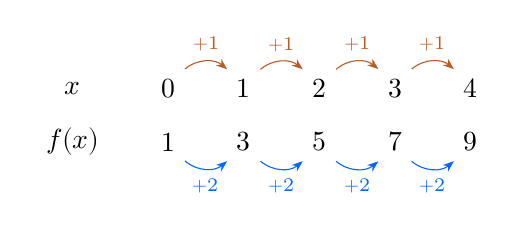
\begin{tikzpicture}
\matrix[column sep=0.55cm,row sep=0.15cm,nodes={font=\normalsize}] (T) {
\node[font=\bfseries]{$x$}; & \node (x0){$0$}; & \node (x1){$1$}; & \node (x2){$2$}; & \node (x3){$3$}; & \node (x4){$4$};\\
\node[font=\bfseries]{$f(x)$}; & \node (y0){$1$}; & \node (y1){$3$}; & \node (y2){$5$}; & \node (y3){$7$}; & \node (y4){$9$};\\
};
\foreach \a/\b in {0/1,1/2,2/3,3/4}{
  \draw[corange,-{Stealth[length=4pt]}] (x\a.north east) to[bend left=40] node[above,font=\scriptsize]{$+1$} (x\b.north west);
  \draw[cblue,-{Stealth[length=4pt]}] (y\a.south east) to[bend right=40] node[below,font=\scriptsize]{$+2$} (y\b.south west);
}
\end{tikzpicture}
\end{center}

На графиката това изглежда като стълба: една стъпка надясно, две стъпки нагоре.

\begin{center}
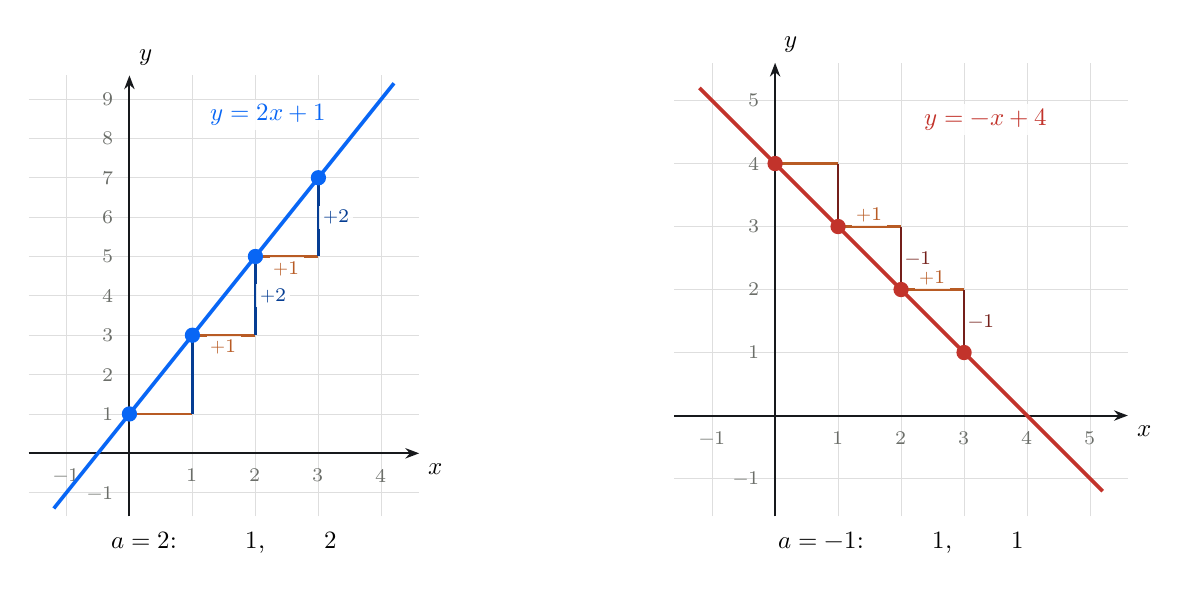
\begin{tikzpicture}
\begin{axis}[fgraph,xmin=-1.6,xmax=4.6,ymin=-1.6,ymax=9.6,x=0.8cm,y=0.5cm,name=A]
\addplot[cblue,domain=-1.2:4.2]{2*x+1};
\foreach \k in {0,1,2}{
  \edef\tmp{\noexpand\draw[corange,line width=1pt] (axis cs:\k,{2*\k+1}) -- (axis cs:{\k+1},{2*\k+1});
            \noexpand\draw[cblue!60!black,line width=1pt] (axis cs:{\k+1},{2*\k+1}) -- (axis cs:{\k+1},{2*\k+3});}\tmp
}
\node[lab,text=corange,below] at (axis cs:1.5,3) {$+1$};
\node[lab,text=cblue!60!black,right] at (axis cs:2,4) {$+2$};
\node[lab,text=corange,below] at (axis cs:2.5,5) {$+1$};
\node[lab,text=cblue!60!black,right] at (axis cs:3,6) {$+2$};
\addplot[pt,cblue] coordinates {(0,1)(1,3)(2,5)(3,7)};
\node[lab,font=\small,anchor=east,text=cblue] at (axis cs:3.2,8.6) {$y=2x+1$};
\end{axis}
\node[font=\small,below=2pt of A,align=center] {$a=2$: надясно $1$, нагоре $2$};
\begin{scope}[xshift=8.2cm]
\begin{axis}[fgraph,xmin=-1.6,xmax=5.6,ymin=-1.6,ymax=5.6,x=0.8cm,y=0.8cm,name=B]
\addplot[cred,domain=-1.2:5.2]{-x+4};
\foreach \k in {0,1,2}{
  \edef\tmp{\noexpand\draw[corange,line width=1pt] (axis cs:\k,{4-\k}) -- (axis cs:{\k+1},{4-\k});
            \noexpand\draw[cred!60!black,line width=1pt] (axis cs:{\k+1},{4-\k}) -- (axis cs:{\k+1},{3-\k});}\tmp
}
\node[lab,text=corange,above] at (axis cs:1.5,3) {$+1$};
\node[lab,text=cred!60!black,right] at (axis cs:2,2.5) {$-1$};
\node[lab,text=corange,above] at (axis cs:2.5,2) {$+1$};
\node[lab,text=cred!60!black,right] at (axis cs:3,1.5) {$-1$};
\addplot[pt,cred] coordinates {(0,4)(1,3)(2,2)(3,1)};
\node[lab,font=\small,anchor=west,text=cred] at (axis cs:2.3,4.7) {$y=-x+4$};
\end{axis}
\node[font=\small,below=2pt of B,align=center] {$a=-1$: надясно $1$, надолу $1$};
\end{scope}
\end{tikzpicture}
\end{center}

\begin{defbox}[Наклон]
Числото $a$ казва \textbf{с колко се променя изходът, когато входът нарасне с $1$}. Нарича се \textbf{наклон}. В училище ще го срещнеш и като „ъглов коефициент“.
\end{defbox}

Знакът на $a$ решава накъде върви правата, когато се движим надясно:

\begin{center}
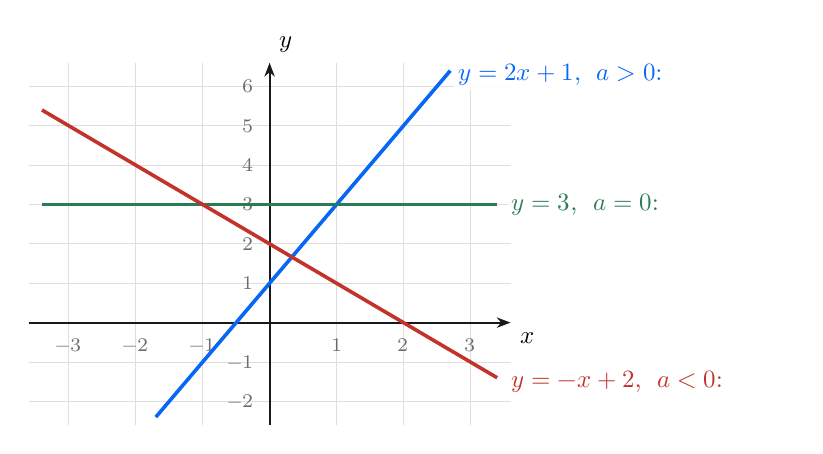
\begin{tikzpicture}
\begin{axis}[fgraph,xmin=-3.6,xmax=3.6,ymin=-2.6,ymax=6.6,x=0.85cm,y=0.5cm]
\addplot[cblue,domain=-1.7:2.7]{2*x+1};
\addplot[cgreen,domain=-3.4:3.4]{3};
\addplot[cred,domain=-3.4:3.4]{-x+2};
\node[lab,font=\small,text=cblue,anchor=west] at (axis cs:2.75,6.3) {$y=2x+1$,\; $a>0$: расте};
\node[lab,font=\small,text=cgreen,anchor=west] at (axis cs:3.55,3) {$y=3$,\; $a=0$: не се променя};
\node[lab,font=\small,text=cred,anchor=west] at (axis cs:3.55,-1.5) {$y=-x+2$,\; $a<0$: намалява};
\end{axis}
\end{tikzpicture}
\end{center}

Колкото по-голямо е $a$, толкова по-стръмна е правата.

\subsection{Какво прави числото \texorpdfstring{$b$}{b}: начало}

Ако сложим $x=0$, получаваме $f(0)=a\cdot 0+b=b$. Значи $b$ е \textbf{мястото, където графиката пресича оста $y$}.
Ако сменим само $b$, правата се мести нагоре или надолу, без да променя наклона си.

На лявата картинка всички прави минават през една точка и се различават само по наклона. На дясната са успоредни и се различават само по $b$.

\begin{center}
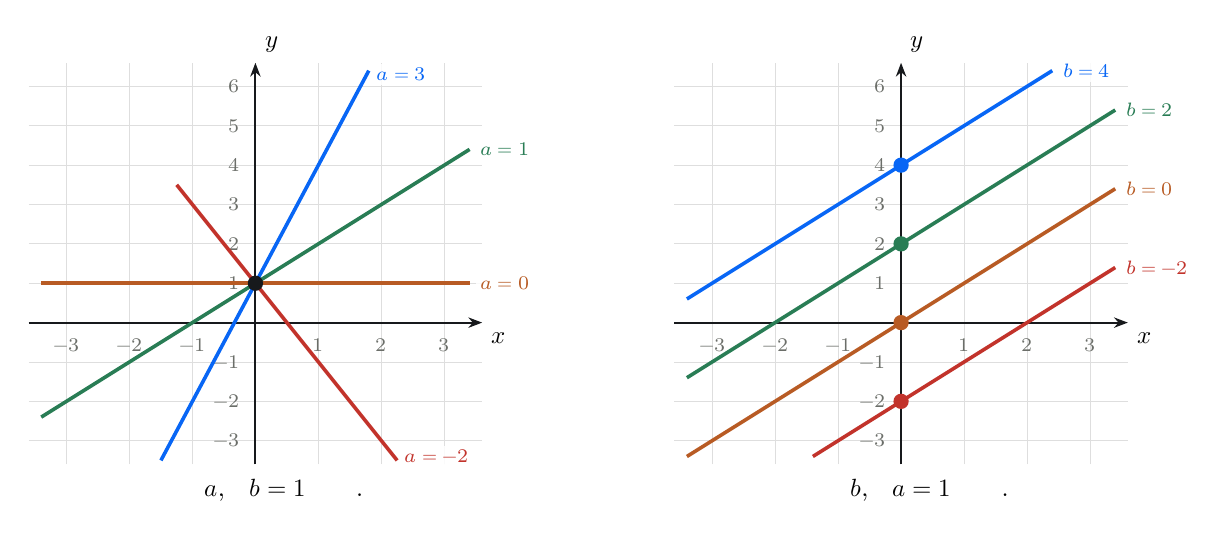
\begin{tikzpicture}
\begin{axis}[fgraph,xmin=-3.6,xmax=3.6,ymin=-3.6,ymax=6.6,x=0.8cm,y=0.5cm,name=A]
\addplot[cred,domain=-1.25:2.25]{-2*x+1}; 
\addplot[corange,domain=-3.4:3.4]{1};
\addplot[cgreen,domain=-3.4:3.4]{x+1};
\addplot[cblue,domain=-1.5:1.8]{3*x+1};
\addplot[pt,ink] coordinates {(0,1)};
\node[lab,text=cblue,anchor=west] at (axis cs:1.85,6.3) {$a=3$};
\node[lab,text=cgreen,anchor=west] at (axis cs:3.5,4.4) {$a=1$};
\node[lab,text=corange,anchor=west] at (axis cs:3.5,1) {$a=0$};
\node[lab,text=cred,anchor=west] at (axis cs:2.3,-3.4) {$a=-2$};
\end{axis}
\node[font=\small,below=2pt of A] {Сменяме $a$, а $b=1$ остава.};
\begin{scope}[xshift=8.2cm]
\begin{axis}[fgraph,xmin=-3.6,xmax=3.6,ymin=-3.6,ymax=6.6,x=0.8cm,y=0.5cm,name=B]
\addplot[cblue,domain=-3.4:2.4]{x+4};
\addplot[cgreen,domain=-3.4:3.4]{x+2};
\addplot[corange,domain=-3.4:3.4]{x};
\addplot[cred,domain=-1.4:3.4]{x-2};
\addplot[pt,cblue] coordinates {(0,4)};\addplot[pt,cgreen] coordinates {(0,2)};
\addplot[pt,corange] coordinates {(0,0)};\addplot[pt,cred] coordinates {(0,-2)};
\node[lab,text=cblue,anchor=west] at (axis cs:2.5,6.4) {$b=4$};
\node[lab,text=cgreen,anchor=west] at (axis cs:3.5,5.4) {$b=2$};
\node[lab,text=corange,anchor=west] at (axis cs:3.5,3.4) {$b=0$};
\node[lab,text=cred,anchor=west] at (axis cs:3.5,1.4) {$b=-2$};
\end{axis}
\node[font=\small,below=2pt of B] {Сменяме $b$, а $a=1$ остава.};
\end{scope}
\end{tikzpicture}
\end{center}

\subsection{Как намираме правилото}

Често знаем няколко стойности, а търсим формулата. Това е същото, което прави един модел, когато се учи от данни.

\textbf{От таблица.}
\begin{center}
\renewcommand{\arraystretch}{1.2}
\begin{tabular}{>{\bfseries}c|*{4}{>{\centering\arraybackslash}p{0.8cm}}}
$x$ & $0$ & $1$ & $2$ & $3$\\\hline
$y$ & $3$ & $5$ & $7$ & $9$
\end{tabular}
\end{center}
При $x=0$ изходът е $3$, значи $b=3$. При всяка стъпка изходът расте с $2$, значи $a=2$. Правилото е $y=2x+3$.
Проверка: $2\cdot 3+3=9$.

\textbf{От две точки.} Правата минава през $(1,4)$ и $(3,10)$.
Входът е нараснал с $3-1=2$, а изходът с $10-4=6$. За една стъпка това са $6:2=3$, значи $a=3$.
\[ a = \frac{10-4}{3-1} = \frac{6}{2} = 3 \]
Сега търсим $b$. Знаем, че $y=3x+b$ и че при $x=1$ изходът е $4$: \; $3\cdot 1+b=4$, значи $b=1$.
Правилото е $y=3x+1$. Проверка с другата точка: $3\cdot 3+1=10$.

\subsection{Линейни функции около нас}

\begin{minipage}[t]{0.5\textwidth}
\textbf{Такси.} Началната такса е $3$ евро, а всеки километър струва $2$ евро. Цената за $x$ километра е
\[ c(x)=2x+3 \]
За $5$ км плащаме $c(5)=2\cdot 5+3=13$ евро.

\vspace{4pt}
\textbf{Свещ.} Свещ е висока $20$ см и всеки час става с $2$ см по-ниска. Височината ѝ в сантиметри след $t$ часа е
\[ h(t)=20-2t \]
Тук наклонът е $-2$, затова графиката слиза. Свещта изгаря, когато $h(t)=0$, тоест при $t=10$ часа.
\end{minipage}\hfill
\begin{minipage}[t]{0.46\textwidth}
\vspace{0pt}
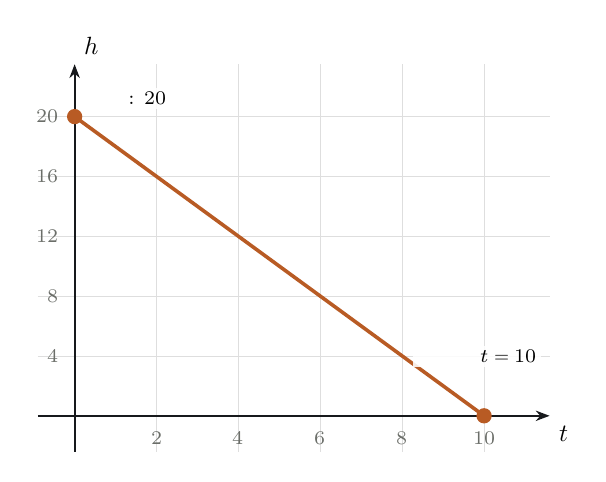
\begin{tikzpicture}
\begin{axis}[fgraph,xmin=-0.9,xmax=11.6,ymin=-2.4,ymax=23.5,x=0.52cm,y=0.19cm,
  xtick distance=2,ytick distance=4,xlabel={$t$},ylabel={$h$}]
\addplot[corange,domain=0:10]{20-2*x};
\addplot[pt,corange] coordinates {(0,20)(10,0)};
\node[lab,anchor=west] at (axis cs:0.4,21.2) {начало: $20$ см};
\node[lab,anchor=south east] at (axis cs:11.4,3.2) {изгаря при $t=10$};
\end{axis}
\end{tikzpicture}
\end{minipage}

Точката, в която графиката пресича оста $x$, се нарича \textbf{нула на функцията}. Там изходът е $0$.
Намираме я, като решим уравнението $ax+b=0$. Това уравнение вече го решавахме на Python в първия урок.

\begin{pybox}
\begin{Verbatim}
def line(x, a, b):
    return a * x + b

print(line(5, 2, 3))      # 13   таксито: a = 2, b = 3
print(line(10, -2, 20))   # 0    свещта: a = -2, b = 20
\end{Verbatim}
Една функция описва всички прави. Числата \texttt{a} и \texttt{b}, които избират коя точно, се наричат \textbf{параметри}.
\end{pybox}

\begin{board}
$f(x)=ax+b$ \quad графиката е права линия\\[2pt]
$a$ = наклон: с колко се променя $y$, когато $x$ нарасне с $1$. \quad $a>0$ расте, $a<0$ намалява.\\[2pt]
$b=f(0)$: където правата пресича оста $y$.\\[2pt]
През две точки: $a=\dfrac{\text{промяна на } y}{\text{промяна на } x}$, после намираме $b$ от едната точка.
\end{board}

\begin{trybox}
\begin{enumerate}[label=\textbf{\arabic*.},start=7]
  \item Какъв е наклонът на $y=5x-7$? Расте ли функцията или намалява?
  \item Къде правата $y=-3x+4$ пресича оста $y$?
  \item Права минава през $(0,2)$ и $(1,5)$. Коя е функцията?
  \item Таксито от примера е взело $21$ евро. Колко километра е пътувал клиентът?
\end{enumerate}
\end{trybox}

% =====================================================================
\section{Квадратна функция}

Какво става, ако повдигнем входа на квадрат?
\[ f(x)=x^2 \]

\begin{minipage}[c]{0.5\textwidth}
\begin{center}
\renewcommand{\arraystretch}{1.2}
\begin{tabular}{>{\bfseries}c|*{7}{>{\centering\arraybackslash}p{0.5cm}}}
$x$ & $-3$ & $-2$ & $-1$ & $0$ & $1$ & $2$ & $3$\\\hline
$x^2$ & $9$ & $4$ & $1$ & $0$ & $1$ & $4$ & $9$
\end{tabular}
\end{center}

Три неща се виждат веднага:
\begin{itemize}
  \item Изходът никога не е отрицателен, защото минус по минус дава плюс.
  \item Числата $-3$ и $3$ дават един и същ изход. Графиката е огледална спрямо оста $y$.
  \item Най-малката стойност е $0$ и се получава при $x=0$.
\end{itemize}
Графиката се нарича \textbf{парабола}, а най-ниската ѝ точка се нарича \textbf{връх}.
\end{minipage}\hfill
\begin{minipage}[c]{0.46\textwidth}
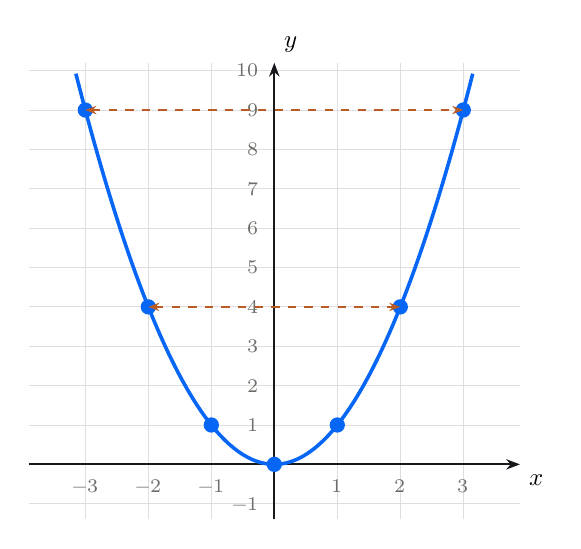
\begin{tikzpicture}
\begin{axis}[fgraph,xmin=-3.9,xmax=3.9,ymin=-1.4,ymax=10.2,x=0.8cm,y=0.5cm]
\addplot[cblue,domain=-3.15:3.15]{x^2};
\addplot[pt,cblue] coordinates {(-3,9)(-2,4)(-1,1)(0,0)(1,1)(2,4)(3,9)};
\draw[corange,dashed,line width=.9pt,{Stealth[length=4pt]}-{Stealth[length=4pt]}] (axis cs:-2,4) -- (axis cs:2,4);
\draw[corange,dashed,line width=.9pt,{Stealth[length=4pt]}-{Stealth[length=4pt]}] (axis cs:-3,9) -- (axis cs:3,9);
\node[lab,text=cgreen,anchor=north west] at (axis cs:0.25,-0.25) {връх};
\end{axis}
\end{tikzpicture}
\end{minipage}

\subsection{Наклонът вече не е един и същ}

При правата всяка стъпка надясно променя изхода с едно и също число. При параболата не е така:

\begin{center}
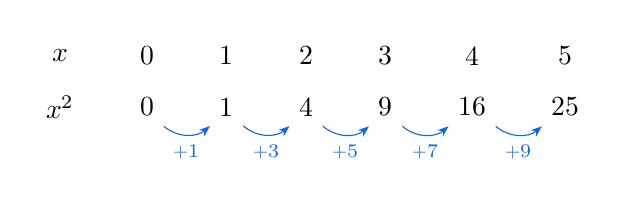
\begin{tikzpicture}
\matrix[column sep=0.6cm,row sep=0.15cm,nodes={font=\normalsize}] (T) {
\node[font=\bfseries]{$x$}; & \node (x0){$0$}; & \node (x1){$1$}; & \node (x2){$2$}; & \node (x3){$3$}; & \node (x4){$4$}; & \node (x5){$5$};\\
\node[font=\bfseries]{$x^2$}; & \node (y0){$0$}; & \node (y1){$1$}; & \node (y2){$4$}; & \node (y3){$9$}; & \node (y4){$16$}; & \node (y5){$25$};\\
};
\foreach \a/\b/\d in {0/1/1,1/2/3,2/3/5,3/4/7,4/5/9}{
  \draw[cblue,-{Stealth[length=4pt]}] (y\a.south east) to[bend right=40] node[below,font=\scriptsize]{$+\d$} (y\b.south west);
}
\end{tikzpicture}
\end{center}

Стъпките са $1, 3, 5, 7, 9$. Близо до нулата параболата е почти равна, а колкото по-далеч отиваме, толкова по-стръмна става.

\subsection{Как се мести параболата}

Малка промяна във формулата мести цялата графика. На четирите картинки сивата линия е $y=x^2$. Едно квадратче е една единица.

\begin{center}
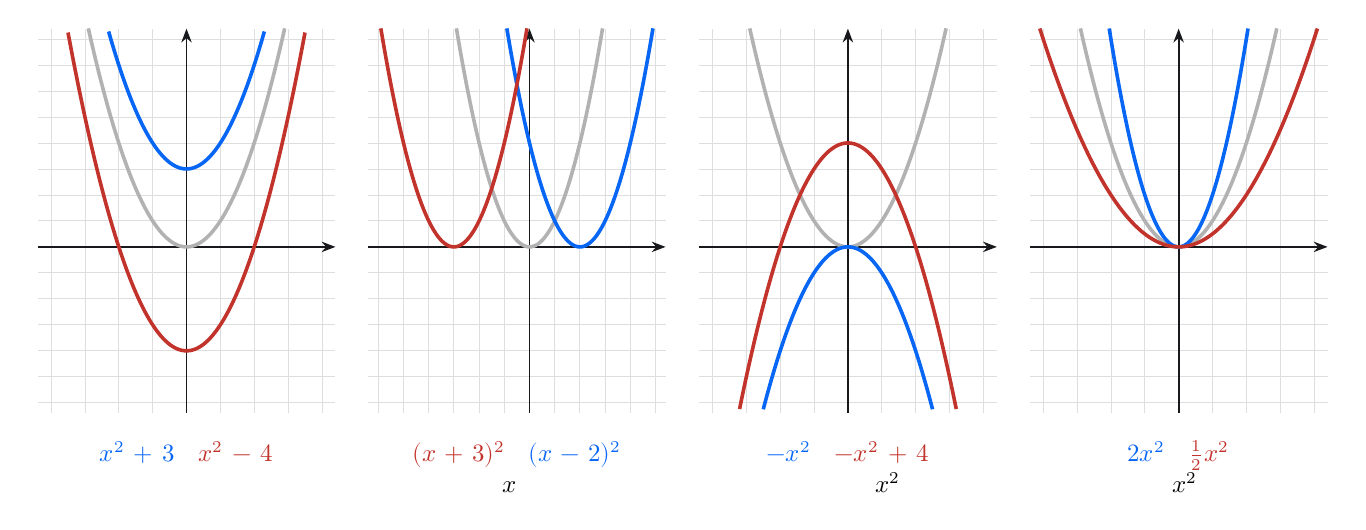
\begin{tikzpicture}
\begin{axis}[fgraph,mini,xmin=-4.4,xmax=4.4,ymin=-6.4,ymax=8.4,name=A,x=0.43cm,y=0.33cm,xticklabels={},yticklabels={},xlabel={},ylabel={}]
\addplot[black!30,domain=-2.9:2.9]{x^2};
\addplot[cblue,domain=-2.3:2.3]{x^2+3};
\addplot[cred,domain=-3.5:3.5]{x^2-4};
\end{axis}
\node[font=\small,below=3pt of A,align=center,text width=3.8cm] {\textbf{Нагоре и надолу}\\\textcolor{cblue}{$x^2+3$} \; \textcolor{cred}{$x^2-4$}\\прибавяме число накрая};
\begin{scope}[xshift=4.2cm]
\begin{axis}[fgraph,mini,xmin=-6.4,xmax=5.4,ymin=-6.4,ymax=8.4,name=B,x=0.32cm,y=0.33cm,xticklabels={},yticklabels={},xlabel={},ylabel={}]
\addplot[black!30,domain=-2.9:2.9]{x^2};
\addplot[cblue,domain=-0.9:4.9]{(x-2)^2};
\addplot[cred,domain=-5.9:-0.1]{(x+3)^2};
\end{axis}
\node[font=\small,below=3pt of B,align=center,text width=3.8cm] {\textbf{Наляво и надясно}\\\textcolor{cred}{$(x+3)^2$} \; \textcolor{cblue}{$(x-2)^2$}\\сменяме $x$ в скобата};
\end{scope}
\begin{scope}[xshift=8.4cm]
\begin{axis}[fgraph,mini,xmin=-4.4,xmax=4.4,ymin=-6.4,ymax=8.4,name=C,x=0.43cm,y=0.33cm,xticklabels={},yticklabels={},xlabel={},ylabel={}]
\addplot[black!30,domain=-2.9:2.9]{x^2};
\addplot[cblue,domain=-2.5:2.5]{-x^2};
\addplot[cred,domain=-3.2:3.2]{-x^2+4};
\end{axis}
\node[font=\small,below=3pt of C,align=center,text width=3.8cm] {\textbf{Обръщане}\\\textcolor{cblue}{$-x^2$} \; \textcolor{cred}{$-x^2+4$}\\минус пред $x^2$};
\end{scope}
\begin{scope}[xshift=12.6cm]
\begin{axis}[fgraph,mini,xmin=-4.4,xmax=4.4,ymin=-6.4,ymax=8.4,name=D,x=0.43cm,y=0.33cm,xticklabels={},yticklabels={},xlabel={},ylabel={}]
\addplot[black!30,domain=-2.9:2.9]{x^2};
\addplot[cblue,domain=-2.05:2.05]{2*x^2};
\addplot[cred,domain=-4.1:4.1]{0.5*x^2};
\end{axis}
\node[font=\small,below=3pt of D,align=center,text width=3.8cm] {\textbf{Тясна и широка}\\\textcolor{cblue}{$2x^2$} \; \textcolor{cred}{$\frac{1}{2}x^2$}\\умножаваме $x^2$ по число};
\end{scope}
\end{tikzpicture}
\end{center}

Защо $(x-2)^2$ се мести \textbf{надясно}, а не наляво? Най-малката стойност на един квадрат е $0$. Тя се получава, когато скобата е нула, тоест при $x=2$. Значи върхът е при $x=2$.

\subsection{Една парабола отблизо}

Да разгледаме $f(x)=x^2-2x-3$. Първо правим таблица:

\begin{center}
\renewcommand{\arraystretch}{1.2}
\begin{tabular}{>{\bfseries}c|*{7}{>{\centering\arraybackslash}p{0.55cm}}}
$x$ & $-2$ & $-1$ & $0$ & $1$ & $2$ & $3$ & $4$\\\hline
$f(x)$ & $5$ & $0$ & $-3$ & $-4$ & $-3$ & $0$ & $5$
\end{tabular}
\end{center}

\begin{minipage}[c]{0.5\textwidth}
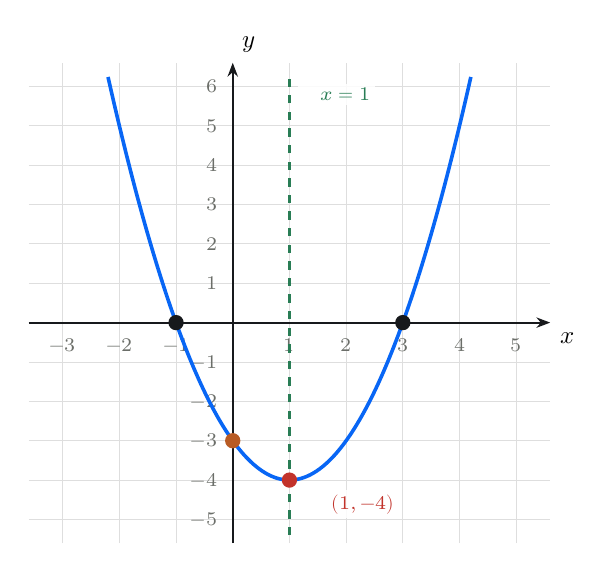
\begin{tikzpicture}
\begin{axis}[fgraph,xmin=-3.6,xmax=5.6,ymin=-5.6,ymax=6.6,x=0.72cm,y=0.5cm]
\addplot[cblue,domain=-2.2:4.2]{x^2-2*x-3};
\draw[cgreen,dashed,line width=.9pt] (axis cs:1,-5.4) -- (axis cs:1,6.4);
\addplot[pt,cred] coordinates {(1,-4)};
\addplot[pt,ink] coordinates {(-1,0)(3,0)};
\addplot[pt,corange] coordinates {(0,-3)};
\node[lab,text=cred,anchor=north west] at (axis cs:1.15,-4.25) {връх $(1,-4)$};
\node[lab,anchor=north east] at (axis cs:-1.2,-0.3) {нула};
\node[lab,anchor=north west] at (axis cs:3.2,-0.3) {нула};
\node[lab,text=cgreen,anchor=west] at (axis cs:1.15,5.8) {ос $x=1$};
\end{axis}
\end{tikzpicture}
\end{minipage}\hfill
\begin{minipage}[c]{0.47\textwidth}
От таблицата и графиката четем:
\begin{itemize}
  \item \textbf{\textcolor{cred}{Връх}} $(1,-4)$. Най-малката стойност на функцията е $-4$.
  \item \textbf{Нули} при $x=-1$ и $x=3$. Там графиката пресича оста $x$.
  \item \textbf{\textcolor{corange}{Пресича оста $y$}} в $-3$, защото $f(0)=-3$.
  \item \textbf{\textcolor{cgreen}{Ос на симетрия}} $x=1$. Тя е точно по средата между двете нули: $\dfrac{-1+3}{2}=1$.
\end{itemize}
\end{minipage}

\subsection{Най-малка и най-голяма стойност}

\begin{minipage}[c]{0.55\textwidth}
Ако пред $x^2$ има плюс, параболата е отворена нагоре и има \textbf{най-малка} стойност (минимум).
Ако има минус, тя е отворена надолу и има \textbf{най-голяма} стойност (максимум).

\vspace{4pt}
\textbf{Пример.} Хвърляме топка нагоре. Височината ѝ в метри след $t$ секунди е $h(t)=-t^2+4t$.

\begin{center}
\renewcommand{\arraystretch}{1.2}
\begin{tabular}{>{\bfseries}c|*{5}{>{\centering\arraybackslash}p{0.5cm}}}
$t$ & $0$ & $1$ & $2$ & $3$ & $4$\\\hline
$h(t)$ & $0$ & $3$ & $4$ & $3$ & $0$
\end{tabular}
\end{center}
Топката стига най-високо след $2$ секунди, на $4$ метра. След $4$ секунди пада на земята.
\end{minipage}\hfill
\begin{minipage}[c]{0.4\textwidth}
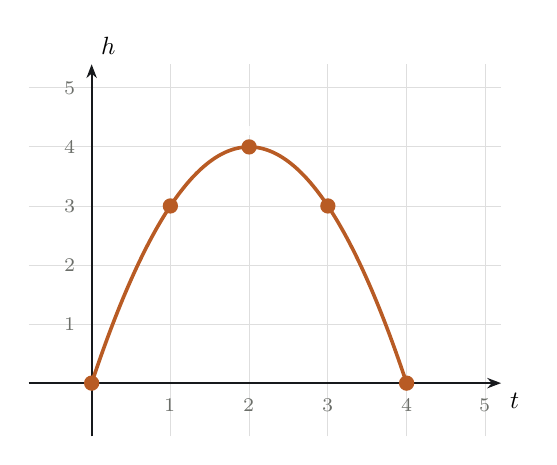
\begin{tikzpicture}
\begin{axis}[fgraph,xmin=-0.8,xmax=5.2,ymin=-0.9,ymax=5.4,x=1.0cm,y=0.75cm,xlabel={$t$},ylabel={$h$}]
\addplot[corange,domain=0:4]{-x^2+4*x};
\addplot[pt,corange] coordinates {(0,0)(1,3)(2,4)(3,3)(4,0)};
\node[lab,anchor=south] at (axis cs:2,4.2) {максимум};
\end{axis}
\end{tikzpicture}
\end{minipage}

\begin{board}
$f(x)=x^2$: парабола, връх в $(0,0)$, огледална спрямо оста $y$.\\[2pt]
$x^2+3$ нагоре, $x^2-4$ надолу, $(x-2)^2$ надясно, $-x^2$ обърната.\\[2pt]
Нули: където $f(x)=0$. \quad Връх: най-ниската или най-високата точка.
\end{board}

\begin{trybox}
\begin{enumerate}[label=\textbf{\arabic*.},start=11]
  \item Къде е върхът на $y=x^2+5$? А на $y=(x-4)^2$?
  \item За кои $x$ е вярно $x^2-4=0$?
  \item Има ли функцията $y=-x^2+9$ най-малка или най-голяма стойност? Колко е тя?
\end{enumerate}
\end{trybox}
% =====================================================================
\section{Зоопарк от функции}

Правите и параболите са само началото. Ето още няколко функции, които се срещат често. За всяка гледай формата на графиката: тя казва как се държи функцията.

% ---------- модул ----------
\subsection{Модул: \texorpdfstring{$f(x)=|x|$}{|x|}}
\begin{minipage}[c]{0.36\textwidth}
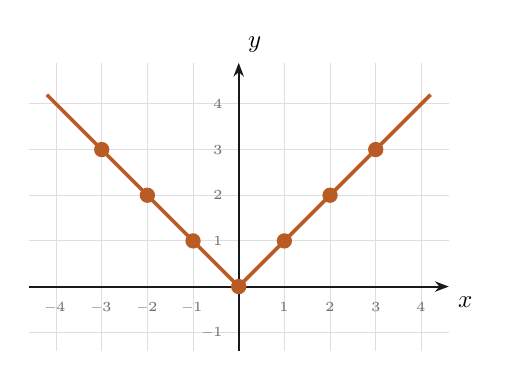
\begin{tikzpicture}
\begin{axis}[fgraph,mini,xmin=-4.6,xmax=4.6,ymin=-1.4,ymax=4.9,x=0.58cm,y=0.58cm]
\addplot[corange,domain=-4.2:4.2,sharp plot,samples=3]{abs(x)};
\addplot[pt,corange] coordinates {(-3,3)(-2,2)(-1,1)(0,0)(1,1)(2,2)(3,3)};
\end{axis}
\end{tikzpicture}
\end{minipage}\hfill
\begin{minipage}[c]{0.6\textwidth}
Модулът е разстоянието от числото до нулата, затова никога не е отрицателен.
\begin{center}
\renewcommand{\arraystretch}{1.15}
\begin{tabular}{>{\bfseries}c|*{7}{>{\centering\arraybackslash}p{0.45cm}}}
$x$ & $-3$ & $-2$ & $-1$ & $0$ & $1$ & $2$ & $3$\\\hline
$|x|$ & $3$ & $2$ & $1$ & $0$ & $1$ & $2$ & $3$
\end{tabular}
\end{center}
Графиката е буква „V“: до нулата слиза с наклон $-1$, след нулата се качва с наклон $1$. В нулата има остър ъгъл.
\end{minipage}

% ---------- куб ----------
\subsection{Куб: \texorpdfstring{$f(x)=x^3$}{x^3}}
\begin{minipage}[c]{0.36\textwidth}
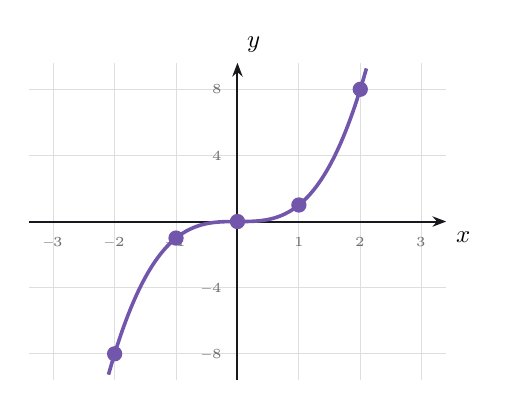
\begin{tikzpicture}
\begin{axis}[fgraph,mini,xmin=-3.4,xmax=3.4,ymin=-9.6,ymax=9.6,x=0.78cm,y=0.21cm,ytick distance=4]
\addplot[cpurple,domain=-2.1:2.1]{x^3};
\addplot[pt,cpurple] coordinates {(-2,-8)(-1,-1)(0,0)(1,1)(2,8)};
\end{axis}
\end{tikzpicture}
\end{minipage}\hfill
\begin{minipage}[c]{0.6\textwidth}
Тук отрицателните входове дават отрицателни изходи, защото минус по минус по минус е минус.
\begin{center}
\renewcommand{\arraystretch}{1.15}
\begin{tabular}{>{\bfseries}c|*{5}{>{\centering\arraybackslash}p{0.55cm}}}
$x$ & $-2$ & $-1$ & $0$ & $1$ & $2$\\\hline
$x^3$ & $-8$ & $-1$ & $0$ & $1$ & $8$
\end{tabular}
\end{center}
Функцията расте навсякъде, но около нулата почти спира. Далеч от нулата расте много по-бързо от $x^2$.
\end{minipage}

% ---------- корен ----------
\subsection{Корен: \texorpdfstring{$f(x)=\sqrt{x}$}{sqrt(x)}}
\begin{minipage}[c]{0.46\textwidth}
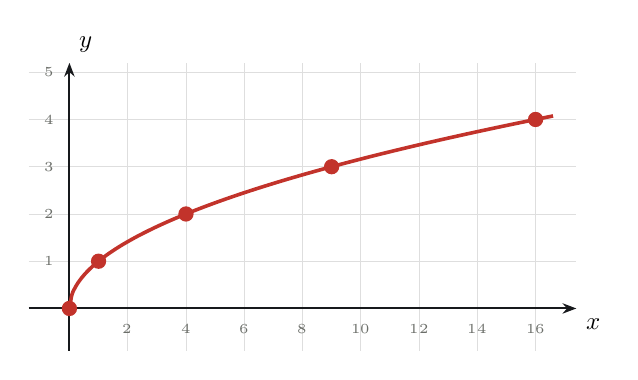
\begin{tikzpicture}
\begin{axis}[fgraph,mini,xmin=-1.4,xmax=17.4,ymin=-0.9,ymax=5.2,x=0.37cm,y=0.6cm,xtick distance=2]
\addplot[cred,domain=0:16.6,samples=200]{sqrt(x)};
\addplot[pt,cred] coordinates {(0,0)(1,1)(4,2)(9,3)(16,4)};
\end{axis}
\end{tikzpicture}
\end{minipage}\hfill
\begin{minipage}[c]{0.5\textwidth}
Коренът е обратното на повдигането на квадрат: $\sqrt{9}=3$, защото $3^2=9$.
\begin{center}
\renewcommand{\arraystretch}{1.15}
\begin{tabular}{>{\bfseries}c|*{5}{>{\centering\arraybackslash}p{0.5cm}}}
$x$ & $0$ & $1$ & $4$ & $9$ & $16$\\\hline
$\sqrt{x}$ & $0$ & $1$ & $2$ & $3$ & $4$
\end{tabular}
\end{center}
Расте все по-бавно. За да стигне от $3$ до $4$, входът трябва да мине от $9$ чак до $16$. Работи само за $x\ge 0$.
\end{minipage}

% ---------- хипербола ----------
\subsection{Обратна пропорционалност: \texorpdfstring{$f(x)=\dfrac{12}{x}$}{12/x}}
\begin{minipage}[c]{0.42\textwidth}
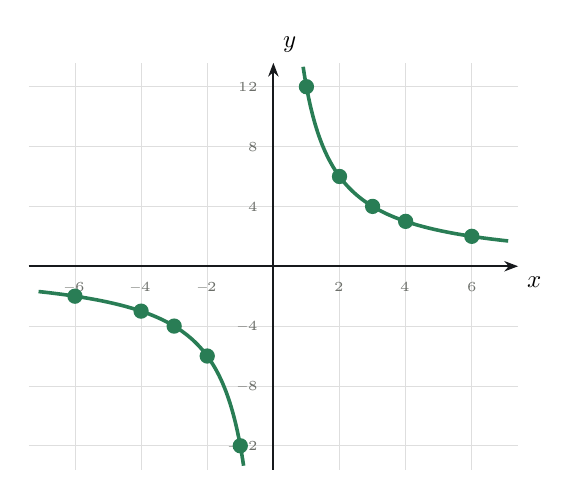
\begin{tikzpicture}
\begin{axis}[fgraph,mini,xmin=-7.4,xmax=7.4,ymin=-13.6,ymax=13.6,x=0.42cm,y=0.19cm,xtick distance=2,ytick distance=4]
\addplot[cgreen,domain=0.9:7.1,samples=200]{12/x};
\addplot[cgreen,domain=-7.1:-0.9,samples=200]{12/x};
\addplot[pt,cgreen] coordinates {(1,12)(2,6)(3,4)(4,3)(6,2)(-1,-12)(-2,-6)(-3,-4)(-4,-3)(-6,-2)};
\end{axis}
\end{tikzpicture}
\end{minipage}\hfill
\begin{minipage}[c]{0.54\textwidth}
Делим $12$ бонбона по равно на $x$ деца. Колкото повече са децата, толкова по-малко получава всяко.
\begin{center}
\renewcommand{\arraystretch}{1.15}
\begin{tabular}{>{\bfseries}c|*{6}{>{\centering\arraybackslash}p{0.5cm}}}
$x$ & $1$ & $2$ & $3$ & $4$ & $6$ & $12$\\\hline
$12/x$ & $12$ & $6$ & $4$ & $3$ & $2$ & $1$
\end{tabular}
\end{center}
Ако входът стане двойно по-голям, изходът става двойно по-малък. При $x=0$ функцията не работи, затова графиката е от две отделни части и никога не докосва осите.
\end{minipage}

% ---------- показателна ----------
\subsection{Удвояване: \texorpdfstring{$f(x)=2^x$}{2^x}}
\begin{minipage}[c]{0.4\textwidth}
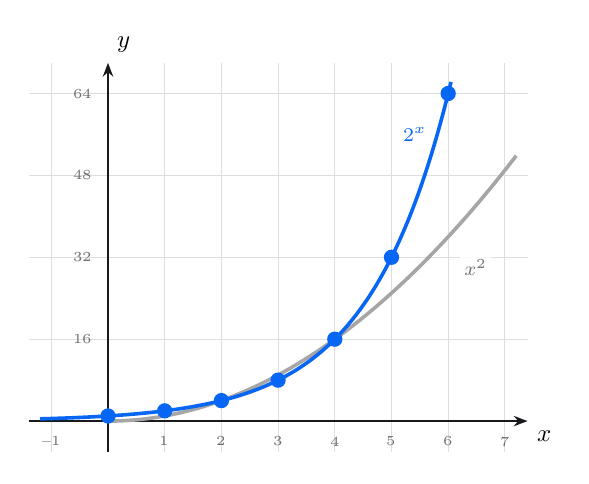
\begin{tikzpicture}
\begin{axis}[fgraph,mini,xmin=-1.4,xmax=7.4,ymin=-6,ymax=70,x=0.72cm,y=0.065cm,ytick distance=16]
\addplot[black!35,domain=0:7.2]{x^2};
\addplot[cblue,domain=-1.2:6.05,samples=200]{2^x};
\addplot[pt,cblue] coordinates {(0,1)(1,2)(2,4)(3,8)(4,16)(5,32)(6,64)};
\node[lab,text=cblue,anchor=east] at (axis cs:5.7,56) {$2^x$};
\node[lab,text=black!55,anchor=west] at (axis cs:6.2,30) {$x^2$};
\end{axis}
\end{tikzpicture}
\end{minipage}\hfill
\begin{minipage}[c]{0.56\textwidth}
Всяка стъпка надясно \textbf{удвоява} изхода. Така растат бактериите, които се делят на две.
\begin{center}
\renewcommand{\arraystretch}{1.15}
\begin{tabular}{>{\bfseries}c|*{7}{>{\centering\arraybackslash}p{0.45cm}}}
$x$ & $0$ & $1$ & $2$ & $3$ & $4$ & $5$ & $6$\\\hline
$2^x$ & $1$ & $2$ & $4$ & $8$ & $16$ & $32$ & $64$
\end{tabular}
\end{center}
В началото изглежда бавна, но после изпреварва всичко. При $x=10$ имаме $x^2=100$, а $2^x=1024$. При $x=20$ имаме $x^2=400$, а $2^x$ е над един милион.
\end{minipage}

\begin{funbox}
Ако сгънеш лист хартия на две $x$ пъти, получаваш $2^x$ пласта. След $10$ сгъвания пластовете са $1024$.
Затова никой не може да сгъне обикновен лист повече от седем или осем пъти.
\end{funbox}

% ---------- стъпаловидна ----------
\subsection{Стъпаловидна функция}
\begin{minipage}[c]{0.4\textwidth}
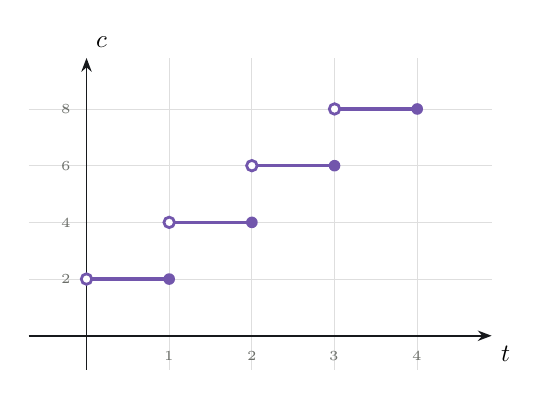
\begin{tikzpicture}
\begin{axis}[fgraph,mini,xmin=-0.7,xmax=4.9,ymin=-1.2,ymax=9.8,x=1.05cm,y=0.36cm,ytick distance=2,xlabel={$t$},ylabel={$c$}]
\foreach \k in {0,1,2,3}{
  \edef\tmp{\noexpand\draw[cpurple,line width=1.3pt] (axis cs:\k,{2*\k+2}) -- (axis cs:{\k+1},{2*\k+2});
  \noexpand\draw[cpurple,line width=1pt,fill=white] (axis cs:\k,{2*\k+2}) circle [radius=1.9pt];
  \noexpand\fill[cpurple] (axis cs:{\k+1},{2*\k+2}) circle [radius=2.1pt];}\tmp
}
\end{axis}
\end{tikzpicture}
\end{minipage}\hfill
\begin{minipage}[c]{0.56\textwidth}
Паркинг взима $2$ евро за всеки \textbf{започнат} час. За $30$ минути плащаш $2$ евро, за точно $1$ час пак $2$, а за $1$ час и $1$ минута вече $4$.

Графиката е стълба. Плътната точка значи „тази стойност се включва“, а празната значи „не се включва“. При $t=1$ цената е $2$, не $4$.

Това пак е функция: за всяко време има точно една цена.
\end{minipage}

% ---------- ReLU ----------
\subsection{Функция на парчета: ReLU}
\begin{minipage}[c]{0.4\textwidth}
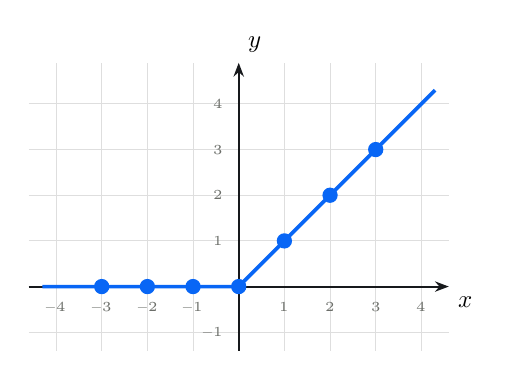
\begin{tikzpicture}
\begin{axis}[fgraph,mini,xmin=-4.6,xmax=4.6,ymin=-1.4,ymax=4.9,x=0.58cm,y=0.58cm]
\addplot[cblue,sharp plot] coordinates {(-4.3,0)(0,0)(4.3,4.3)};
\addplot[pt,cblue] coordinates {(-3,0)(-2,0)(-1,0)(0,0)(1,1)(2,2)(3,3)};
\end{axis}
\end{tikzpicture}
\end{minipage}\hfill
\begin{minipage}[c]{0.56\textwidth}
Някои функции имат различно правило за различни входове:
\[ r(x)=\begin{cases} x, & \text{ако } x>0\\ 0, & \text{ако } x\le 0\end{cases} \]
Положителните числа минават непроменени, а отрицателните стават $0$. Например $r(3)=3$ и $r(-3)=0$.

Тази функция се казва \textbf{ReLU} и е една от най-използваните в невронните мрежи.
\end{minipage}

\begin{pybox}
\begin{Verbatim}
def relu(x):
    if x > 0:
        return x
    return 0

print(relu(3), relu(-3))    # 3 0
\end{Verbatim}
„Функция на парчета“ в математиката е функция с \texttt{if} в Python.
\end{pybox}

% ---------- без формула ----------
\subsection{Функция без формула: сума на цифрите}

Не всяка функция се записва с формула. В първия урок писахме програма за сумата на цифрите на число.
Това също е функция: на всяко число съпоставя точно една сума. Например $S(2026)=2+0+2+6=10$.

\begin{center}
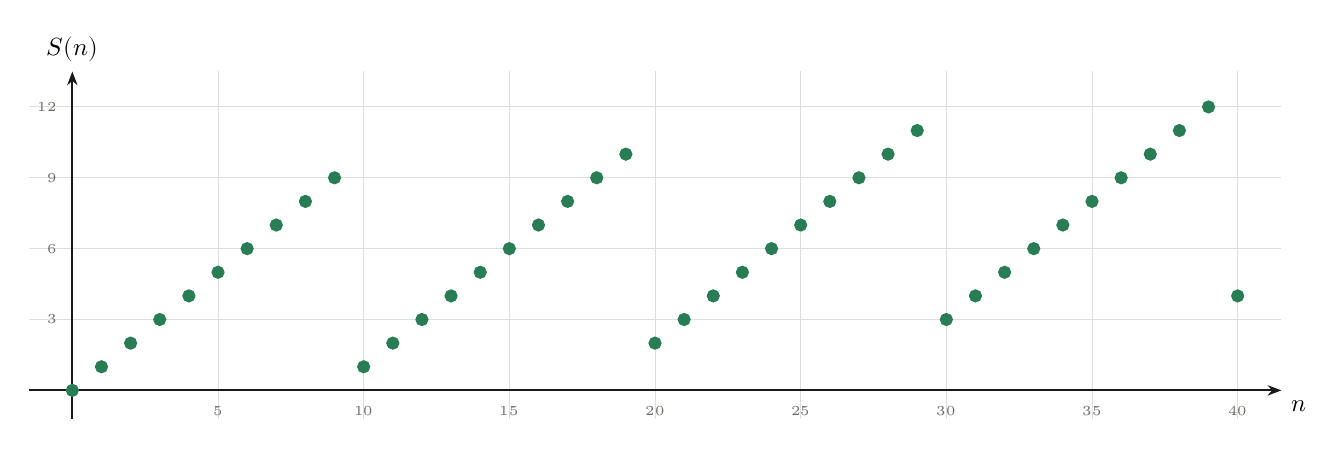
\begin{tikzpicture}
\begin{axis}[fgraph,mini,xmin=-1.5,xmax=41.5,ymin=-1.2,ymax=13.5,x=0.37cm,y=0.3cm,xtick distance=5,ytick distance=3,xlabel={$n$},ylabel={$S(n)$},
  ylabel style={at={(ticklabel* cs:1)},anchor=south,font=\small}]
\addplot[pt,cgreen,mark size=1.7pt] coordinates {
(0,0)(1,1)(2,2)(3,3)(4,4)(5,5)(6,6)(7,7)(8,8)(9,9)
(10,1)(11,2)(12,3)(13,4)(14,5)(15,6)(16,7)(17,8)(18,9)(19,10)
(20,2)(21,3)(22,4)(23,5)(24,6)(25,7)(26,8)(27,9)(28,10)(29,11)
(30,3)(31,4)(32,5)(33,6)(34,7)(35,8)(36,9)(37,10)(38,11)(39,12)(40,4)};
\end{axis}
\end{tikzpicture}
\end{center}

Графиката е от отделни точки, защото входовете са само цели числа. Сумата расте с $1$ и на всеки десет числа пада рязко.

\begin{funbox}[За любопитните: задача, която никой не е решил]
Вземи цяло положително число. Ако е четно, раздели го на $2$. Ако е нечетно, умножи го по $3$ и прибави $1$. Повтаряй.

Започваме от $6$: \quad $6 \to 3 \to 10 \to 5 \to 16 \to 8 \to 4 \to 2 \to 1$.

Досега всяко проверено число накрая стига до $1$. Никой обаче не е доказал, че това е вярно за всички числа. Правилото е толкова просто, че се пише с пет реда на Python.
\end{funbox}

\begin{board}
$|x|$: буква „V“, винаги $\ge 0$. \qquad $x^3$: и отрицателни изходи.\\[2pt]
$\sqrt{x}$: само за $x\ge 0$, расте все по-бавно. \qquad $\dfrac{12}{x}$: не работи при $x=0$.\\[2pt]
$2^x$: удвоява се на всяка стъпка: $1, 2, 4, 8, 16, \dots$\\[2pt]
ReLU: $r(x)=x$ при $x>0$, иначе $0$.
\end{board}

\begin{trybox}
\begin{enumerate}[label=\textbf{\arabic*.},start=14]
  \item Колко е $|{-5}|+|2|$? А $\sqrt{36}$? А $(-1)^3$?
  \item Бактерия се дели на две всеки час. В началото е една. Колко са след $5$ часа?
  \item Колко е $r(-7)+r(7)$, където $r$ е ReLU?
\end{enumerate}
\end{trybox}

% =====================================================================
\section{Какво ни казва графиката}

Когато гледаме графика, четем я \textbf{отляво надясно}, както четем текст.

\subsection{Расте или намалява}

\begin{minipage}[c]{0.46\textwidth}
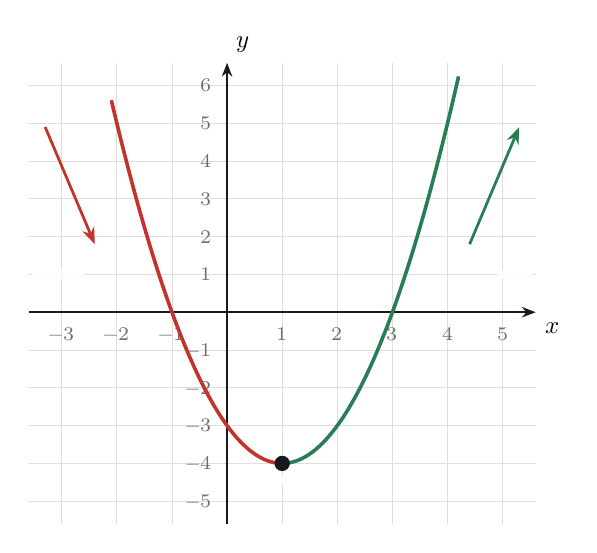
\begin{tikzpicture}
\begin{axis}[fgraph,xmin=-3.6,xmax=5.6,ymin=-5.6,ymax=6.6,x=0.7cm,y=0.48cm]
\addplot[cred,domain=-2.1:1]{x^2-2*x-3};
\addplot[cgreen,domain=1:4.2]{x^2-2*x-3};
\addplot[pt,ink] coordinates {(1,-4)};
\draw[cred,-{Stealth[length=6pt]},line width=1pt] (axis cs:-3.3,4.9) -- (axis cs:-2.4,1.8);
\draw[cgreen,-{Stealth[length=6pt]},line width=1pt] (axis cs:4.4,1.8) -- (axis cs:5.3,4.9);
\node[lab,text=cred,anchor=west] at (axis cs:-3.55,1.0) {намалява};
\node[lab,text=cgreen,anchor=east] at (axis cs:5.55,1.0) {расте};
\node[lab,anchor=north] at (axis cs:1,-4.3) {минимум};
\end{axis}
\end{tikzpicture}
\end{minipage}\hfill
\begin{minipage}[c]{0.5\textwidth}
Функцията \textbf{\textcolor{cgreen}{расте}}, когато графиката се качва при движение надясно: по-голям вход дава по-голям изход.

Функцията \textbf{\textcolor{cred}{намалява}}, когато графиката слиза.

На картинката е $f(x)=x^2-2x-3$. До $x=1$ тя намалява, а след $x=1$ расте. Точката, в която слизането се сменя с качване, е \textbf{минимумът}.

Правата расте или намалява навсякъде. Параболата прави и двете.
\end{minipage}

\subsection{Симетрия}

Някои графики са симетрични и това личи и във формулата.

\begin{center}
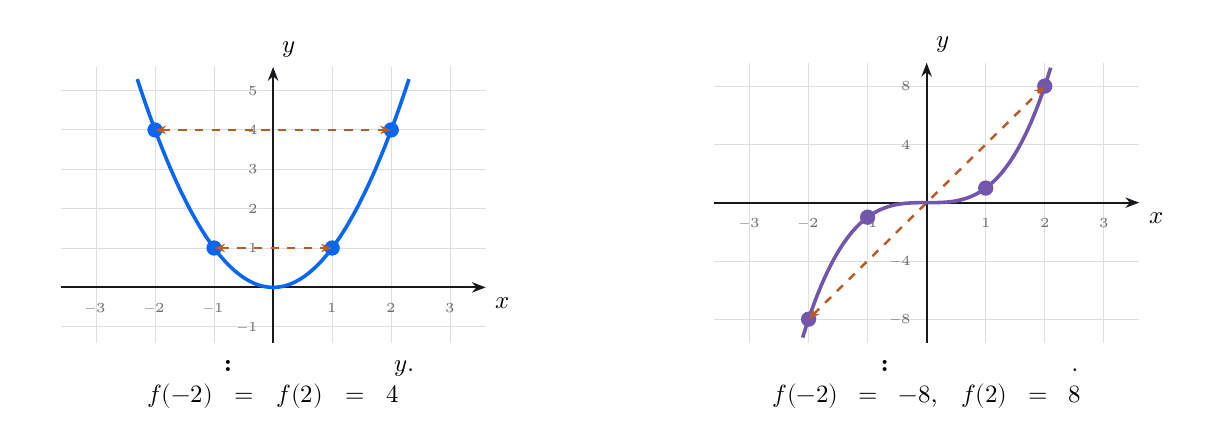
\begin{tikzpicture}
\begin{axis}[fgraph,mini,xmin=-3.6,xmax=3.6,ymin=-1.4,ymax=5.6,x=0.75cm,y=0.5cm,name=A]
\addplot[cblue,domain=-2.3:2.3]{x^2};
\addplot[pt,cblue] coordinates {(-2,4)(2,4)(-1,1)(1,1)};
\draw[corange,dashed,line width=.9pt,{Stealth[length=4pt]}-{Stealth[length=4pt]}] (axis cs:-2,4) -- (axis cs:2,4);
\draw[corange,dashed,line width=.9pt,{Stealth[length=4pt]}-{Stealth[length=4pt]}] (axis cs:-1,1) -- (axis cs:1,1);
\end{axis}
\node[font=\small,below=3pt of A,align=center,text width=6cm] {\textbf{Четна функция:} огледало спрямо оста $y$.\\$f(-2)=f(2)=4$};
\begin{scope}[xshift=8.3cm]
\begin{axis}[fgraph,mini,xmin=-3.6,xmax=3.6,ymin=-9.6,ymax=9.6,x=0.75cm,y=0.185cm,ytick distance=4,name=B]
\addplot[cpurple,domain=-2.1:2.1]{x^3};
\addplot[pt,cpurple] coordinates {(-2,-8)(2,8)(-1,-1)(1,1)};
\draw[corange,dashed,line width=.9pt,{Stealth[length=4pt]}-{Stealth[length=4pt]}] (axis cs:-2,-8) -- (axis cs:2,8);
\end{axis}
\node[font=\small,below=3pt of B,align=center,text width=6.4cm] {\textbf{Нечетна функция:} завъртане около началото.\\$f(-2)=-8$, а $f(2)=8$};
\end{scope}
\end{tikzpicture}
\end{center}

\begin{itemize}
  \item \textbf{Четна} функция: срещуположните входове дават един и същ изход, $f(-x)=f(x)$. Примери: $x^2$, $|x|$, $x^2-4$.
  \item \textbf{Нечетна} функция: срещуположните входове дават срещуположни изходи, $f(-x)=-f(x)$. Примери: $x$, $x^3$, $\dfrac{12}{x}$.
  \item Повечето функции не са нито едното, нито другото. Например $f(x)=2x+1$: $f(2)=5$, а $f(-2)=-3$.
\end{itemize}

За да провериш, сметни $f(2)$ и $f(-2)$ и ги сравни.

\begin{board}
Четем графиката отляво надясно: качва се = расте, слиза = намалява.\\[2pt]
Минимум и максимум: където посоката се сменя.\\[2pt]
Четна: $f(-x)=f(x)$, огледало спрямо оста $y$. \quad Нечетна: $f(-x)=-f(x)$.
\end{board}

\begin{trybox}
\begin{enumerate}[label=\textbf{\arabic*.},start=17]
  \item Четна, нечетна или нито едно от двете е $f(x)=x^2+1$? А $g(x)=x+3$?
  \item За кои $x$ расте функцията $y=|x|$?
\end{enumerate}
\end{trybox}

% =====================================================================
\section{Функция от функция}

Какво става, ако изходът на една машинка влезе в друга?

Нека $f(x)=x+3$ и $g(x)=2x$. Пускаме $1$ първо през $f$, после през $g$:

\begin{center}
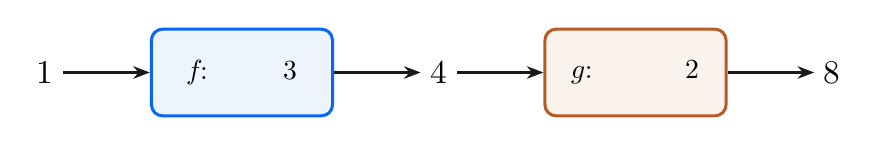
\begin{tikzpicture}
\node[io] (in) at (0,0) {$1$};
\node[mach,minimum width=2.3cm,minimum height=1.1cm,right=1.1cm of in] (f) {$f$: прибави $3$};
\node[io,right=1.1cm of f] (mid) {$4$};
\node[mach,minimum width=2.3cm,minimum height=1.1cm,right=1.1cm of mid,draw=corange,fill=corange!8] (g) {$g$: умножи по $2$};
\node[io,right=1.1cm of g] (out) {$8$};
\draw[arr] (in) -- (f); \draw[arr] (f) -- (mid); \draw[arr] (mid) -- (g); \draw[arr] (g) -- (out);
\end{tikzpicture}
\end{center}

Записваме го така: $g(f(1))=g(4)=8$. Чете се отвътре навън: първо смятаме вътрешната скоба.

Редът има значение. Ако разменим машинките, получаваме $f(g(1))=f(2)=5$.

\begin{pybox}
\begin{Verbatim}
def f(x):
    return x + 3

def g(x):
    return 2 * x

print(g(f(1)))    # 8
print(f(g(1)))    # 5
\end{Verbatim}
Точно такива въпроси имаше в урок 3: какво отпечатва \texttt{add(add(1, 1), 1)}.
\end{pybox}

\begin{board}
$f(x)=x+3$, \; $g(x)=2x$\\[2pt]
$g(f(1))=g(4)=8$ \qquad $f(g(1))=f(2)=5$ \qquad Смятаме отвътре навън. Редът има значение.
\end{board}

\begin{trybox}
\begin{enumerate}[label=\textbf{\arabic*.},start=19]
  \item Нека $f(x)=x+1$ и $g(x)=3x$. Колко е $g(f(2))$? А $f(g(2))$?
\end{enumerate}
\end{trybox}

% =====================================================================
\section{Функциите и изкуственият интелект}

\begin{minipage}[c]{0.44\textwidth}
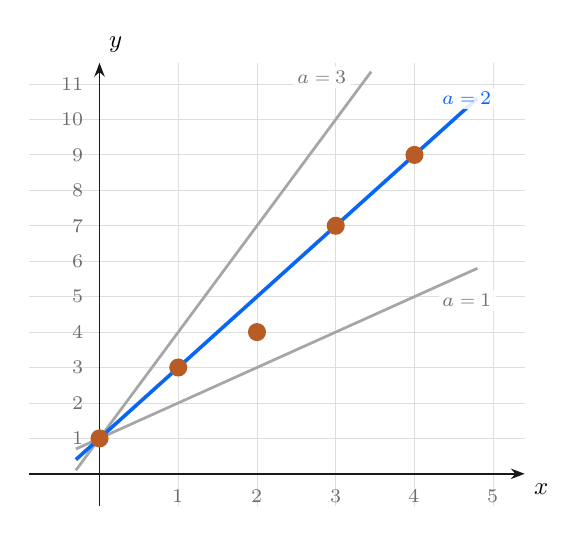
\begin{tikzpicture}
\begin{axis}[fgraph,xmin=-0.9,xmax=5.4,ymin=-0.9,ymax=11.6,x=1.0cm,y=0.45cm]
\addplot[black!35,domain=-0.3:4.8,line width=1pt]{x+1};
\addplot[black!35,domain=-0.3:3.45,line width=1pt]{3*x+1};
\addplot[cblue,domain=-0.3:4.8]{2*x+1};
\addplot[pt,corange,mark size=2.6pt] coordinates {(0,1)(1,3)(2,4)(3,7)(4,9)};
\node[lab,text=black!55,anchor=west] at (axis cs:4.3,4.9) {$a=1$};
\node[lab,text=cblue,anchor=west] at (axis cs:4.3,10.6) {$a=2$};
\node[lab,text=black!55,anchor=east] at (axis cs:3.2,11.2) {$a=3$};
\end{axis}
\end{tikzpicture}
\end{minipage}\hfill
\begin{minipage}[c]{0.52\textwidth}
Оранжевите точки са \textbf{данни}: измерени входове и изходи. Не знаем правилото, което ги свързва.

Избираме вид функция, например $y=ax+b$. Това е \textbf{моделът}. Числата $a$ и $b$ са неговите \textbf{параметри}.

\textbf{Обучението} е търсене на тези $a$ и $b$, при които правата минава най-близо до точките. Тук синята права с $a=2$ и $b=1$ е най-добра.
\end{minipage}

\vspace{4pt}
Същото направихме в урок 3 с ябълките и крушите. Там моделът беше правило с един параметър, прага, и програмата намери най-добрия праг от данните.

Големите модели, с които говорим всеки ден, също са функции. Те са съставени от огромен брой прости функции, пуснати една след друга: линейни функции и ReLU. Параметрите им са милиарди, но идеята е същата.

% =====================================================================
\section{Всичко на едно място}

\begin{center}
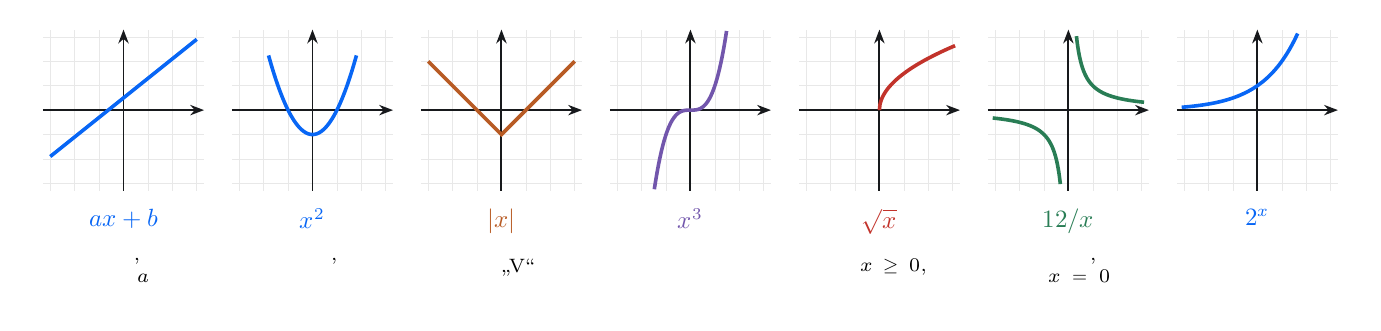
\begin{tikzpicture}
\newcommand{\thumb}[5]{%
\begin{scope}[xshift=#1cm]
\begin{axis}[fgraph,xmin=-3.3,xmax=3.3,ymin=-3.3,ymax=3.3,x=0.31cm,y=0.31cm,xticklabels={},yticklabels={},xlabel={},ylabel={},
  grid style={line width=.2pt,draw=black!9},name=T]
#4
\end{axis}
\node[font=\small\bfseries,below=3pt of T,text=#5] {#2};
\node[font=\scriptsize,below=21pt of T,align=center,text width=2.2cm] {#3};
\end{scope}}
\thumb{0}{$ax+b$}{права,\\наклон $a$}{\addplot[cblue,domain=-3:3]{0.8*x+0.5};}{cblue}
\thumb{2.4}{$x^2$}{парабола,\\има връх}{\addplot[cblue,domain=-1.8:1.8]{x^2-1};}{cblue}
\thumb{4.8}{$|x|$}{буква „V“}{\addplot[corange,domain=-3:3,sharp plot,samples=3]{abs(x)-1};}{corange}
\thumb{7.2}{$x^3$}{расте\\навсякъде}{\addplot[cpurple,domain=-1.48:1.48]{x^3};}{cpurple}
\thumb{9.6}{$\sqrt{x}$}{само $x\ge 0$,\\расте бавно}{\addplot[cred,domain=0:3.1,samples=150]{1.5*sqrt(x)};}{cred}
\thumb{12.0}{$12/x$}{две части,\\без $x=0$}{\addplot[cgreen,domain=0.33:3.1,samples=100]{1/x};\addplot[cgreen,domain=-3.1:-0.33,samples=100]{1/x};}{cgreen}
\thumb{14.4}{$2^x$}{удвояване}{\addplot[cblue,domain=-3.1:1.65,samples=100]{2^x};}{cblue}
\end{tikzpicture}
\end{center}

\begin{itemize}
  \item \textbf{Функция:} правило, което на всеки вход дава точно един изход. Записваме $f(x)$.
  \item \textbf{Графика:} всички точки $(x,f(x))$. От нея четем стойности, нули, минимум и максимум, къде функцията расте.
  \item \textbf{Линейна функция} $ax+b$: $a$ е наклонът, $b$ е стойността при $x=0$.
  \item \textbf{Параметри:} числата във формулата, които избираме. Моделите в изкуствения интелект са функции с много параметри.
\end{itemize}

% =====================================================================
\needspace{7cm}
\section*{Отговори на „Провери се“}\label{sec:answers}
\addcontentsline{toc}{section}{Отговори на „Провери се“}
{\small
\begin{multicols}{2}
\begin{enumerate}[label=\textbf{\arabic*.},leftmargin=2em]
  \item $g(3)=8$, $g(0)=-1$, $g(-3)=8$.
  \item $x=4$.
  \item Да. Всяко число има точно едно следващо.
  \item $f(-2)=-2$, $f(0)=2$, $f(3)=2$.
  \item $x=-3$, $x=-1$ и $x=4$.
  \item $4$, при $x=2$.
  \item Наклонът е $5$. Функцията расте.
  \item В точката $(0,4)$.
  \item $y=3x+2$.
  \item $2x+3=21$, значи $x=9$ километра.
  \item $(0,5)$ и $(4,0)$.
  \item $x=2$ и $x=-2$.
  \item Най-голяма стойност: $9$, при $x=0$.
  \item $7$, \; $6$, \; $-1$.
  \item $2^5=32$.
  \item $0+7=7$.
  \item $f$ е четна. $g$ не е нито четна, нито нечетна.
  \item За $x>0$.
  \item $g(f(2))=g(3)=9$, \; $f(g(2))=f(6)=7$.
\end{enumerate}
\end{multicols}}
% =====================================================================
\newpage
\section*{Задачи за часа}
\addcontentsline{toc}{section}{Задачи за часа}

Във всички задачи отговорите са цели числа. Ако получиш дроб, провери сметките си.
Задачите със звезда \st{} са по-трудни.

\grp{А}{Вход и изход}
\begin{tasks}
  \item Нека $f(x)=3x-2$. Намери $f(0)$, $f(1)$, $f(4)$ и $f(-2)$.
  \item Нека $g(x)=x^2+1$. Намери $g(0)$, $g(2)$, $g(-2)$ и $g(5)$.
  \item Нека $h(x)=10-2x$. За кое $x$ е вярно $h(x)=0$? А $h(x)=4$?
  \item Попълни таблицата за $f(x)=2x-3$.
  \begin{center}\renewcommand{\arraystretch}{1.3}
  \begin{tabular}{>{\bfseries}c|*{6}{>{\centering\arraybackslash}p{0.9cm}}}
  $x$ & $-1$ & $0$ & $1$ & $2$ & $3$ & $4$\\\hline
  $f(x)$ & & & & & &
  \end{tabular}\end{center}
  \item Кои от тези правила са функции?
  \begin{enumerate}[label=\bgalph*)]
    \item На всяко число съпоставяме неговия модул.
    \item На всяко положително число съпоставяме число, чийто модул е то.
    \item Таблицата \; \begin{tabular}{c|ccc} $x$ & $1$ & $2$ & $3$\\\hline $y$ & $5$ & $5$ & $5$\end{tabular}
    \item Таблицата \; \begin{tabular}{c|ccc} $x$ & $1$ & $1$ & $2$\\\hline $y$ & $3$ & $4$ & $5$\end{tabular}
  \end{enumerate}
\end{tasks}

\grp{Б}{Графики}
\begin{tasks}
  \needspace{6cm}
  \item На картинката е графиката на функция $g$.

  \begin{minipage}[c]{0.4\textwidth}
  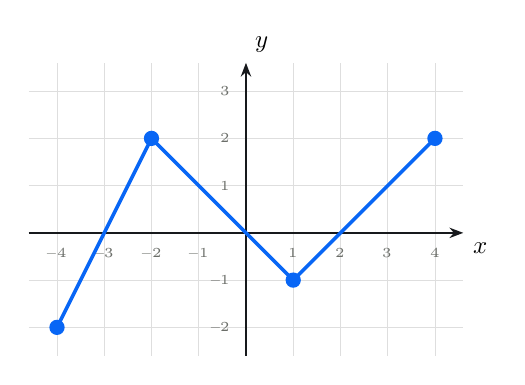
\begin{tikzpicture}
  \begin{axis}[fgraph,mini,xmin=-4.6,xmax=4.6,ymin=-2.6,ymax=3.6,x=0.6cm,y=0.6cm]
  \addplot[cblue,sharp plot] coordinates {(-4,-2)(-2,2)(1,-1)(4,2)};
  \addplot[pt,cblue] coordinates {(-4,-2)(-2,2)(1,-1)(4,2)};
  \end{axis}
  \end{tikzpicture}
  \end{minipage}\hfill
  \begin{minipage}[c]{0.56\textwidth}
  \begin{enumerate}[label=\bgalph*)]
    \item Намери $g(-2)$, $g(0)$, $g(1)$ и $g(3)$.
    \item За кои $x$ е вярно $g(x)=0$?
    \item За кои $x$ е вярно $g(x)=2$?
    \item Коя е най-малката стойност на функцията?
    \item За кои $x$ функцията намалява?
  \end{enumerate}
  \end{minipage}

  \needspace{5cm}
  \item Кои от тези линии са графики на функции?
  \begin{center}
  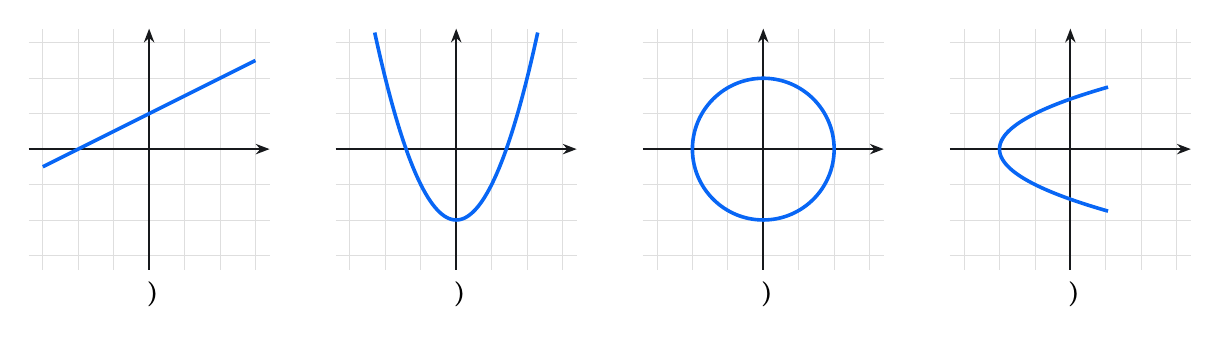
\begin{tikzpicture}
  \foreach \i/\lbl in {0/а,1/б,2/в,3/г}{
  \begin{scope}[xshift=\i*3.9cm]
  \begin{axis}[fgraph,mini,xmin=-3.4,xmax=3.4,ymin=-3.4,ymax=3.4,x=0.45cm,y=0.45cm,xticklabels={},yticklabels={},xlabel={},ylabel={},name=P]
  \ifnum\i=0 \addplot[cblue,domain=-3:3]{0.5*x+1};\fi
  \ifnum\i=1 \addplot[cblue,domain=-2.3:2.3]{x^2-2};\fi
  \ifnum\i=2 \draw[cblue,line width=1.3pt] (axis cs:0,0) circle [radius=2];\fi
  \ifnum\i=3 \addplot[cblue,domain=-1.75:1.75,samples=80,variable=\t] ({\t*\t-2},{\t});\fi
  \end{axis}
  \node[font=\small\bfseries,below=1pt of P] {\lbl)};
  \end{scope}}
  \end{tikzpicture}
  \end{center}

  \item Направи таблица за $f(x)=x-2$ при $x=-2,-1,0,1,2,3,4$ и начертай графиката в тетрадката си.
\end{tasks}

\grp{В}{Линейни функции}
\begin{tasks}
  \item За всяка функция кажи колко са $a$ и $b$ и дали функцията расте, намалява или не се променя.
  \begin{multicols}{4}
  \begin{enumerate}[label=\bgalph*)]
    \item $y=5x-7$
    \item $y=-3x+4$
    \item $y=6$
    \item $y=x$
  \end{enumerate}
  \end{multicols}
  \item Намери правилото $y=ax+b$ за всяка таблица.

  \begin{tabular}{c|cccc} $x$ & $0$ & $1$ & $2$ & $3$\\\hline $y$ & $4$ & $7$ & $10$ & $13$\end{tabular}
  \hspace{1.5cm}
  \begin{tabular}{c|cccc} $x$ & $0$ & $1$ & $2$ & $3$\\\hline $y$ & $9$ & $7$ & $5$ & $3$\end{tabular}
  \item Намери линейната функция, чиято графика минава през двете точки.
  \begin{multicols}{3}
  \begin{enumerate}[label=\bgalph*)]
    \item $(0,2)$ и $(1,5)$
    \item $(1,4)$ и $(3,10)$
    \item \st{} $(2,1)$ и $(4,-3)$
  \end{enumerate}
  \end{multicols}
  \item Къде графиката пресича оста $y$ и къде пресича оста $x$?
  \begin{multicols}{2}
  \begin{enumerate}[label=\bgalph*)]
    \item $y=2x-6$
    \item $y=-x+5$
  \end{enumerate}
  \end{multicols}
  \item Такси има начална такса $3$ евро и взима по $2$ евро на километър.
  \begin{enumerate}[label=\bgalph*)]
    \item Напиши функцията $c(x)$ за цената на $x$ километра.
    \item Колко струват $5$ километра?
    \item Клиент е платил $21$ евро. Колко километра е пътувал?
  \end{enumerate}
  \item Свещ е висока $20$ см и всеки час става с $2$ см по-ниска.
  \begin{enumerate}[label=\bgalph*)]
    \item Напиши функцията $h(t)$ за височината след $t$ часа.
    \item Колко е висока след $3$ часа?
    \item След колко часа е висока $8$ см?
    \item След колко часа изгаря напълно?
  \end{enumerate}
  \needspace{4cm}
  \item \st{} Два мобилни плана. План А: $10$ евро на месец и по $1$ евро за всеки гигабайт. План Б: $4$ евро на месец и по $3$ евро за всеки гигабайт.
  \begin{enumerate}[label=\bgalph*)]
    \item Напиши двете функции $A(x)$ и $B(x)$ за цената при $x$ гигабайта.
    \item Кой план е по-евтин при $1$ гигабайт? А при $5$?
    \item При колко гигабайта двата плана струват еднакво?
  \end{enumerate}
\end{tasks}

\grp{Г}{Квадратни функции}
\begin{tasks}
  \item Попълни таблицата за $f(x)=x^2-4$. Къде са нулите? Коя е най-малката стойност?
  \begin{center}\renewcommand{\arraystretch}{1.3}
  \begin{tabular}{>{\bfseries}c|*{7}{>{\centering\arraybackslash}p{0.8cm}}}
  $x$ & $-3$ & $-2$ & $-1$ & $0$ & $1$ & $2$ & $3$\\\hline
  $f(x)$ & & & & & & &
  \end{tabular}\end{center}
  \item Свържи всяка графика с формулата ѝ: \quad $x^2+2$, \quad $(x-3)^2$, \quad $-x^2+1$, \quad $x^2-1$.
  \begin{center}
  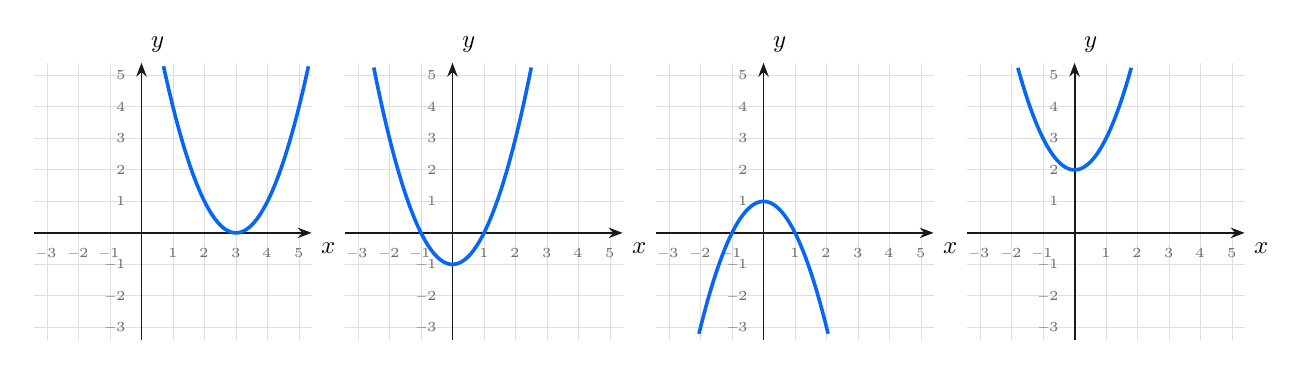
\begin{tikzpicture}
  \foreach \i/\lbl in {0/А,1/Б,2/В,3/Г}{
  \begin{scope}[xshift=\i*3.95cm]
  \begin{axis}[fgraph,mini,xmin=-3.4,xmax=5.4,ymin=-3.4,ymax=5.4,x=0.4cm,y=0.4cm,name=P]
  \ifnum\i=0 \addplot[cblue,domain=0.7:5.3]{(x-3)^2};\fi
  \ifnum\i=1 \addplot[cblue,domain=-2.5:2.5]{x^2-1};\fi
  \ifnum\i=2 \addplot[cblue,domain=-2.05:2.05]{-x^2+1};\fi
  \ifnum\i=3 \addplot[cblue,domain=-1.8:1.8]{x^2+2};\fi
  \end{axis}
  \node[font=\small\bfseries,below=1pt of P] {\lbl};
  \end{scope}}
  \end{tikzpicture}
  \end{center}
  \item Нека $f(x)=x^2-4x+3$.
  \begin{enumerate}[label=\bgalph*)]
    \item Направи таблица за $x=0,1,2,3,4$.
    \item Къде са нулите на функцията?
    \item Къде е върхът?
  \end{enumerate}
  \item Хвърляме топка нагоре. Височината ѝ в метри след $t$ секунди е $h(t)=-t^2+6t$.
  \begin{enumerate}[label=\bgalph*)]
    \item Направи таблица за $t=0,1,2,3,4,5,6$.
    \item Колко е най-голямата височина и кога се достига?
    \item Кога топката пада на земята?
    \item В кои моменти топката е на височина $8$ метра?
  \end{enumerate}
  \item \st{} За кои цели числа $x$ е вярно $x^2<2x+3$? Направи таблица с двете страни за $x$ от $-2$ до $4$.
\end{tasks}

\needspace{5cm}
\grp{Д}{Зоопарк от функции}
\begin{tasks}
  \item Пресметни.

  {\renewcommand{\arraystretch}{1.9}\begin{tabular}{@{\hspace{0.4em}}*{4}{p{0.22\linewidth}}@{}}
  а) $|{-7}|+|3|$ & б) $|2-9|$ & в) $\sqrt{49}$ & г) $\sqrt{9+16}$ \\
  д) $2^5$ & е) $(-2)^3$ & ж) $\dfrac{12}{-4}$ & з) $\sqrt{2^6}$
  \end{tabular}}

  \item Нека $f(x)=|x-3|$. Направи таблица за $x$ от $0$ до $6$. При кое $x$ стойността е най-малка? За кои $x$ е вярно $f(x)=2$?
  \item Бактерия се дели на две всеки час. В началото има една бактерия.
  \begin{enumerate}[label=\bgalph*)]
    \item Колко бактерии има след $10$ часа?
    \item След колко часа бактериите за пръв път са повече от $100$?
  \end{enumerate}
  \item Нека $f(x)=\dfrac{24}{x}$. Намери $f(1)$, $f(2)$, $f(3)$, $f(4)$, $f(6)$, $f(8)$ и $f(-12)$.
  \item Паркинг взима $2$ евро за всеки започнат час. Колко плащаш за:
  \begin{multicols}{4}
  \begin{enumerate}[label=\bgalph*)]
    \item $30$ минути
    \item точно $1$ час
    \item $61$ минути
    \item $3$ часа и $10$ мин
  \end{enumerate}
  \end{multicols}
  \item Нека $r$ е функцията ReLU. Намери $r(5)$, $r(-3)$, $r(0)$ и $r(2)+r(-2)$.
  \item Нека $f(x)=x+3$ и $g(x)=2x$. Намери:
  \begin{multicols}{4}
  \begin{enumerate}[label=\bgalph*)]
    \item $g(f(1))$
    \item $f(g(1))$
    \item $f(f(2))$
    \item $g(g(g(1)))$
  \end{enumerate}
  \end{multicols}
  \item Четна, нечетна или нито едно от двете? Провери с $x=2$ и $x=-2$.

  {\renewcommand{\arraystretch}{1.9}\begin{tabular}{@{\hspace{0.4em}}*{3}{p{0.3\linewidth}}@{}}
  а) $x^2+1$ & б) $x^3$ & в) $|x|$ \\
  г) $2x+1$ & д) $\dfrac{12}{x}$ & е) \st{} $x^3-x$
  \end{tabular}}

  \item \textbf{На Python.} Напиши функцията $f(x)=x^2-4x+3$ с \texttt{def} и отпечатай стойностите ѝ за $x$ от $0$ до $4$ с цикъл. Сравни с таблицата от задача 18.
\end{tasks}

% =====================================================================
\newpage
\section*{Домашно}
\addcontentsline{toc}{section}{Домашно}
\setlist[tasks]{label=\textbf{\arabic*.},leftmargin=2.2em,itemsep=7pt,topsep=4pt}

И тук всички отговори са цели числа. Задачи 1 до 12 са за всички, а останалите са за тези, които искат още.

\begin{tasks}
  \item Нека $f(x)=4x-5$. Намери $f(0)$, $f(2)$ и $f(-1)$. За кое $x$ е вярно $f(x)=7$?
  \item Нека $g(x)=x^2-9$. Намери $g(0)$, $g(3)$, $g(-3)$, $g(4)$ и $g(-5)$.
  \item Намери правилото $y=ax+b$ за всяка таблица.

  \begin{tabular}{c|cccc} $x$ & $0$ & $1$ & $2$ & $3$\\\hline $y$ & $1$ & $5$ & $9$ & $13$\end{tabular}
  \hspace{0.8cm}
  \begin{tabular}{c|cccc} $x$ & $0$ & $1$ & $2$ & $3$\\\hline $y$ & $10$ & $7$ & $4$ & $1$\end{tabular}
  \hspace{0.8cm}
  \begin{tabular}{c|cccc} $x$ & $1$ & $2$ & $3$ & $4$\\\hline $y$ & $5$ & $7$ & $9$ & $11$\end{tabular}
  \item Намери линейната функция, чиято графика минава през двете точки.
  \begin{multicols}{2}
  \begin{enumerate}[label=\bgalph*)]
    \item $(0,-1)$ и $(2,5)$
    \item $(1,6)$ и $(4,0)$
  \end{enumerate}
  \end{multicols}
  \item Начертай в една координатна система графиките на $y=2x-2$ и $y=-x+4$. В коя точка се пресичат?
  \item В басейн има $30$ литра вода. Пълним го с $5$ литра в минута.
  \begin{enumerate}[label=\bgalph*)]
    \item Напиши функцията $V(t)$ за литрите след $t$ минути.
    \item Колко литра има след $4$ минути?
    \item След колко минути литрите са $100$?
  \end{enumerate}
  \item Фитнес зала взима $20$ евро еднократно за карта и по $15$ евро на месец.
  \begin{enumerate}[label=\bgalph*)]
    \item Напиши функцията $c(m)$ за общата цена за $m$ месеца.
    \item Колко струват $6$ месеца?
    \item Някой е платил общо $200$ евро. Колко месеца е ходил?
  \end{enumerate}
  \item Нека $f(x)=x^2-2x$. Направи таблица за $x=-1,0,1,2,3$. Къде са нулите? Къде е върхът?
  \item Нека $f(x)=-x^2+4$. Направи таблица за $x$ от $-3$ до $3$. Коя е най-голямата стойност? За кои цели $x$ функцията е положителна?
  \item Топка е хвърлена нагоре и височината ѝ след $t$ секунди е $h(t)=-t^2+8t$ метра. Колко е най-голямата височина и кога се достига? Кога топката пада на земята? Кога е на $12$ метра?
  \item Пресметни.

  {\renewcommand{\arraystretch}{1.9}\begin{tabular}{@{\hspace{0.4em}}*{4}{p{0.22\linewidth}}@{}}
  а) $|{-12}|-|5|$ & б) $|3-10|$ & в) $\sqrt{81}$ & г) $\sqrt{36+64}$ \\
  д) $2^6$ & е) $(-3)^3$ & ж) $\dfrac{18}{-6}$ & з) $\sqrt{2^4}$
  \end{tabular}}

  \item Нека $f(x)=|x|-2$. Направи таблица за $x$ от $-3$ до $3$ и начертай графиката. Къде са нулите? Коя е най-малката стойност?
  \item Сгъваме лист хартия на две няколко пъти. Колко пласта има след $5$ сгъвания? Колко сгъвания трябват, за да станат пластовете поне $1000$?
  \item Нека $f(x)=x-1$ и $g(x)=x^2$. Намери $g(f(4))$, $f(g(4))$, $g(g(2))$ и $f(f(f(10)))$.
  \item Четна, нечетна или нито едно от двете?
  \begin{multicols}{4}
  \begin{enumerate}[label=\bgalph*)]
    \item $x^2-3$
    \item $x^3+x$
    \item $x+1$
    \item $|x|+2$
  \end{enumerate}
  \end{multicols}
  \item \textbf{На Python.} Напиши с \texttt{def} функциите $f(x)=x^2-2x$ и ReLU. Отпечатай с цикъл стойностите на $f$ за $x$ от $-1$ до $3$ и стойностите на ReLU за $x$ от $-3$ до $3$.
  \item \st{} Машинка работи по неизвестно правило. Знаем само тази таблица. Намери формулата.
  \begin{center}
  \begin{tabular}{c|cccc} вход & $1$ & $2$ & $3$ & $4$\\\hline изход & $3$ & $8$ & $15$ & $24$\end{tabular}
  \end{center}
  \item \st{} Правилото от карето „За любопитните“: ако числото е четно, дели се на $2$, а ако е нечетно, умножава се по $3$ и се прибавя $1$. Започни от $7$ и продължавай, докато стигнеш до $1$. Колко стъпки са нужни? Напиши и програма на Python, която брои стъпките за произволно начално число.
\end{tasks}

\end{document}
